\documentclass[review,3p,authoryear]{elsarticle}

\usepackage{hyperref}
\hypersetup{colorlinks=true,linkcolor=blue,citecolor=blue,urlcolor=blue,hypertexnames=false}
\pdfstringdefDisableCommands{\def\corref#1{}\def\cnotenum{}}%suppress elsarticle bookmark warnings
\usepackage{booktabs}
\usepackage{adjustbox}
\usepackage{tabularx}
\usepackage{amsmath}
\usepackage{amssymb}
\usepackage{graphicx}
\usepackage{multirow}
\usepackage{array}
\usepackage{float}


\journal{Energy Policy}

\bibliographystyle{elsarticle-harv}

\begin{document}

\begin{frontmatter}

\begin{highlights}
\item Renewables are 12.5\% of capacity but only 5.7\% of generation (14 thermal incumbents)
\item Six of seven markets impose zero or negligible carbon prices on power generation
\item Coal emissions do not decline under grow-out as currently practised; under demand growth they increase
\item Coal drag constrains six of fourteen thermal incumbents from scaling clean investment
\item Dispatch reform, PPA renegotiation, managed CF decline, and storage can make grow-out work
\end{highlights}

\title{Growing Out of Coal? Firm-Level Evidence from Emerging Asia}

\author[inst1]{Jose Luis Resendiz\corref{cor1}}
\ead{jose.resendiz@smithschool.ox.ac.uk}

\author[inst1]{Gireesh Shrimali}
\ead{gireesh.shrimali@smithschool.ox.ac.uk}

\cortext[cor1]{Corresponding author}

\affiliation[inst1]{organization={Smith School of Enterprise and the Environment},
            addressline={University of Oxford, South Parks Road},
            city={Oxford},
            postcode={OX1 3QY},
            country={United Kingdom}}

\begin{abstract}
The dominant energy transition strategy in emerging Asia is adding renewable capacity without closing coal plants. No study has tested whether this ``grow out of coal'' strategy actually reduces emissions at the firm level. Using financial and operational data for 20 utilities across seven markets ($\sim$310~GW), we find that it does not. Coal operates at 50--65\% capacity factors versus 20--30\% for solar and wind, so renewables account for 12.5\% of installed capacity but only 5.7\% of generation; demand growth of 5--7\% absorbs new renewable output before it displaces coal; and six of seven markets impose no carbon price on power generation. Coal also creates a financial trap we term ``coal drag'': it funds renewable investment yet constrains the borrowing needed to scale it. These findings show that grow-out succeeds as energy policy but fails as climate policy, because the strategy adds capacity without changing the dispatch, contracts, or price signals that keep coal running. Four mechanisms can close the gap without requiring plant closure: dispatch reform, PPA renegotiation, managed capacity factor decline, and solar-plus-storage deployment. Because the failure is rooted in the gap between MW (capacity) and TWh (generation), transition plans and finance products expressed in MW systematically overstate progress; credibility assessment should be restructured around TWh displacement.
\end{abstract}

\begin{keyword}
energy transition \sep coal phase-out \sep power utilities \sep carbon pricing \sep transition finance \sep emerging Asia
\end{keyword}

\end{frontmatter}

%% ============================================================
%% 1. INTRODUCTION
%% ============================================================
\section{Introduction}

Across Asia's coal-dependent developing economies, the gap between renewable ambition and coal retirement is not a failure of implementation. India's National Electricity Plan targets 500~GW of non-fossil capacity by 2030 but contains no coal retirement schedule \citep{CEA2023}. Indonesia received \$20~billion in JETP commitments in 2022 and then scheduled 6.3~GW of new coal \citep{Ashurst2025}. Vietnam's revised power plan projects rapid renewable expansion, yet EVN grew its coal fleet between 2018 and 2023 with no plant closures disclosed \citep{GIGA2024}. The common strategy is to build renewable capacity without closing coal plants, letting coal's share decline as the system grows. This ``grow out of coal'' approach is the energy transition plan, not a deviation from it. This paper tests whether it works as climate policy: whether it reduces absolute coal generation and emissions at the firm level, and whether the structural conditions for coal displacement are in place. The answer provides a diagnostic basis for evaluating the credibility of utility transition plans and the national targets built on them.

The distinction between energy policy and climate policy is central. As an energy strategy, grow-out is straightforward: expand generation capacity to meet rising demand while keeping coal for grid reliability and energy security. As a climate strategy, however, it must be judged by whether it reduces total coal generation and therefore total CO$_2$ emissions. Coal plants operate at far higher capacity factors than solar or wind; a typical ratio is three to one in annual generation per installed megawatt. If coal plants keep running while renewables are added alongside them, coal's share of the capacity mix falls, but total emissions do not necessarily follow. The question is whether this gap closes at the firm level, where investment decisions are actually made, and whether the structural conditions for it to close are in place.

Three research areas address the problem from different angles but leave the firm-level question open. The displacement literature shows that new energy sources historically add to rather than replace fossil fuels at the country level \citep{York2012,Zhu2017}, but cross-country regressions cannot isolate the firm-level mechanisms. Optimisation models show that coal phase-out \textit{can} be cost-beneficial under ambitious climate targets \citep{NatureComms2025India}, but these prescribe what utilities should do, not what they are doing. The development economics literature on aid fungibility \citep{Feyzioglu1998} warns that earmarked finance can be absorbed without changing behaviour, a risk directly relevant to energy transition investment commitments flowing through thermal incumbents. What is missing across all three is a firm-level diagnostic: no study has examined whether the grow-out calculation actually closes for individual utilities, or systematically assessed whether the structural conditions for coal displacement exist. A recent systematic review of coal phase-out research confirmed this gap, finding no firm-level empirical studies and overwhelming geographic concentration in the UK, US, and Germany \citep{Diluiso2021}.

We address that gap using financial and operational data as of 2023--2024 for 20 utilities across India, Indonesia, Vietnam, Thailand, the Philippines, Malaysia, and Singapore ($\sim$310~GW, covering roughly one-third of on-grid coal capacity in these markets), combined with plant-level capacity data \citep{GEM2026Coal}. We estimate generation from installed capacity using fuel-specific running rates, exposing how the gap between coal and renewable utilisation translates into a gap between capacity shares and generation shares. We develop a firm-level diagnostic framework for evaluating whether the structural conditions for coal displacement are in place, organised along five dimensions: coal retirement pathways~(D1), carbon cost exposure~(D2), technology displacement~(D3), capital reallocation~(D4), and balance sheet resilience~(D5). Dynamic simulations then test whether renewable additions displace coal or are absorbed by rising consumption.

The answer is clear: grow-out as currently practised does not reduce emissions. Across 14 coal-owning utilities ($\sim$161~GW of coal), renewables account for 12.5\% of installed capacity but only 5.7\% of generation. Even doubling every utility's renewable capacity, coal would still provide 67\% of electricity, and total emissions (706~MtCO$_2$/yr) would not fall. Under dynamic simulations with demand growth, emissions increase by roughly 3\% as new renewable output is absorbed by rising consumption rather than replacing coal. Consider the strongest test case: NTPC, India's largest utility (65~GW coal), plans 60~GW of renewables; even with the full pipeline built, coal would still provide 69\% of its generation. Six of seven markets charge nothing or next to nothing for carbon emissions, removing the price signal that would make coal uneconomic. At \$75/tCO$_2$, sixteen of seventeen utilities with fossil generation would face carbon costs exceeding 50\% of EBITDA. Coal exposure also creates a financial double bind we call ``coal drag'': coal provides the revenue that funds renewable expansion, but coal-related debt limits how much utilities can borrow to scale that investment. Across all five diagnostic dimensions, the structural conditions for coal displacement are largely absent: no utility has disclosed plant-level retirement dates, carbon pricing is missing or negligible, technology displacement is minimal, and coal drag constrains the financial capacity to accelerate. Transition plans that assume grow-out will deliver emissions reductions are not supported by the conditions on the ground.

These findings make four contributions to the literature. First, we quantify the capacity factor wedge at the firm level: the relationship between MW additions and TWh displacement that technology-level analyses \citep{Patzek2023} have not applied to individual utilities. Second, we bring the concept of aid fungibility \citep{Feyzioglu1998} into transition finance, showing that financial support for coal-owning utilities can be absorbed without reducing coal generation. Third, we introduce ``coal drag'' as a construct capturing the paradox that coal simultaneously funds and constrains the transition, integrating portfolio lock-in \citep{Alova2020}, the climate investment trap \citep{Ameli2021}, and stranded-asset exposure \citep{CarbonTracker2021}. Fourth, we demonstrate that demand growth of 5--7\% absorbs new renewable generation before it can displace coal, a mechanism that cross-country studies conflate with other factors. The policy implication is that grow-out can work as climate policy, but only if complemented by mechanisms the current strategy omits: dispatch reform to create economic pressure on inefficient coal \citep{Yu2023}, contract renegotiation to reduce lock-in \citep{Boute2025}, managed decline in coal running rates \citep{An2025}, and solar-plus-storage deployment to capture coal's remaining hours. Together, these contributions yield a diagnostic framework for evaluating whether utility transition plans and the national targets built on them are credible. The framework applies to any utility with publicly available capacity data; whether the grow-out calculation closes differently in other regions or at higher carbon prices remains an open question the framework is designed to test.

The remainder of the paper proceeds as follows. Section~\ref{sec:literature} reviews the political economy of grow-out, the displacement gap, and the fungibility problem in transition finance. Section~\ref{sec:methodology} presents the diagnostic design, generation methodology, and data. Section~\ref{sec:results} reports results. Section~\ref{sec:discussion} interprets the findings and discusses policy implications. Section~\ref{sec:conclusion} concludes.

%% ============================================================
%% 2. LITERATURE REVIEW
%% ============================================================
\section{Literature Review}
\label{sec:literature}

This paper engages three literatures: (i) the political economy of coal in emerging Asia, where the question is why coal persists despite cheaper alternatives; (ii) the economics of renewable displacement, where the question is whether adding clean capacity actually reduces fossil generation; and (iii) transition finance design, where the question is whether financial support for coal-owning utilities produces emissions reductions or is absorbed without changing behaviour. Each addresses a different dimension of the grow-out problem, but none tests the strategy empirically at the firm level.

\subsection{Why Coal Persists: Political Economy and Market Structure}

The dominant explanation for coal's persistence in emerging Asia combines political economy constraints with market structure rigidities. Surveys of energy experts across major coal countries find that economic growth, system stability, and cheap electricity consistently outweigh environmental objectives \citep{Ohlendorf2022}. In India, coal demand grows at 5--6\% annually, sustained by fiscal transfers, employment in 51 coal-dependent districts, and regulated tariffs guaranteeing returns on coal assets \citep{Chandra2025,Pai2021}. India is moving \textit{toward} greater coal use, not away from it \citep{Roy2021}; before phase-out, it must first reach a ``plateau of coal'' \citep{Tongia2020}. In Indonesia, coal mining interests and domestic supply obligations mean that the actors resisting coal retirement control the utility itself \citep{Ordonez2021}. In Vietnam, 44\% of experts say central planning rather than market signals drives phase-out decisions \citep{Do2023}.

These political economy forces are reinforced by a contractual framework that locks coal into the generation mix independently of cost. Over 90\% of coal capacity in the markets we study operates under long-term power purchase agreements with take-or-pay clauses, capacity payments, and guaranteed dispatch \citep{Boute2025}. These contracts insulate coal from both market competition and carbon pricing: even where renewables are cheaper, coal plants with contractually guaranteed dispatch face no incentive to reduce output \citep{Bodnar2020}. Coal fleets are also young (10--19 years on average), implying decades of remaining life and elevated stranding exposure \citep{Tong2019,Cui2019,Pfeiffer2016}. None of the 14 coal-owning utilities in our sample has disclosed plant-level retirement dates. The absence of retirement pathways is not a data gap; it is the strategy itself.

\subsection{The Displacement Gap: Why Adding Renewables Does Not Proportionally Reduce Coal}

If coal persists for political and contractual reasons, the grow-out strategy assumes that adding enough renewable capacity will eventually shift the generation mix regardless. A large empirical literature suggests otherwise. \citet{York2012} found that across 130+ nations, each unit of non-fossil energy displaced less than one-quarter of a unit of fossil energy. In China, the ratio is higher but still far below unity \citep{Zhu2017}. The pattern is consistent with energy transitions operating as ``additions'' rather than ``substitutions''.

The capacity factor wedge explains why. Coal operates at 50--65\% capacity factors in the markets we study; solar and wind at 20--30\%. A megawatt of coal therefore produces 2.5--3 times the annual generation of a megawatt of solar or wind, a ratio quantified at the technology level \citep{Patzek2023} but never applied at the utility portfolio level. Even where renewables achieve dispatch priority, they achieve only 91--93\% of theoretically expected displacement because forcing thermal plants to cycle at low capacity factors increases their per-unit emissions \citep{Suri2025}.

Demand growth widens the gap further. In emerging economies with electricity demand growing at 5--7\% annually, new renewable generation is absorbed by incremental consumption rather than displacing coal. Four-fifths of global emissions carry no carbon price, and the average effective rate is below \$3/tCO$_2$ \citep{Rafaty2025}, removing the signal that would force coal off the merit order. The displacement literature uses panel regressions that conflate demand growth with other mechanisms; no study isolates demand-growth absorption as a firm-level variable.

\subsection{Transition Finance and the Fungibility Problem}

The political economy and displacement literatures explain why coal persists and why renewables do not automatically displace it. A third literature raises a different question: even if transition finance is directed at the problem, does it change the outcome? The development economics literature established decades ago that earmarked aid is fungible: recipients substitute aided spending for expenditure they would have undertaken regardless \citep{Feyzioglu1998,Devarajan2000}. This framework has not been applied to climate transition finance, despite mounting evidence that the same dynamic operates. Indonesia received \$20~billion in JETP commitments in 2022, yet PLN went on to schedule 6.3~GW of new coal while backloading 70\% of renewable additions to post-2030 \citep{Ashurst2025}. Globally, over \$200~billion has been allocated for coal phase-out compensation with flows directed largely to governments or utilities rather than linked to plant-level milestones \citep{Nacke2024}. \citet{Boute2025} documents that JETP early retirement schemes risk compensating coal PPA holders in full without requiring verified closure.

The financial structure of coal-owning utilities compounds the fungibility risk. Higher borrowing costs in emerging markets delay clean investment even where strategic intent exists \citep{Ameli2021}. Among 3,000+ utilities worldwide, portfolio composition rather than ownership determines transition outcomes, and three-quarters did not meaningfully shift portfolios over two decades \citep{Alova2020}. Coal-heavy utilities face a financial double bind: coal generates the cash flow funding renewable expansion while simultaneously constraining the balance sheet to scale it. Individual components of this mechanism have been documented separately: portfolio lock-in \citep{Alova2020}, the country-level climate investment trap \citep{Ameli2021}, structural destabilisation of European incumbents \citep{Kungl2018}, and stranded-asset exposure \citep{CarbonTracker2021}. No study has integrated these into a unified firm-level framework.

\subsection{What Is Missing}

The three literatures converge on a common implication but leave it untested. Coal persists because political economy and contracts protect it. Renewables do not displace it because capacity factors and demand growth absorb new generation. Transition finance does not change this because it flows through the same utilities whose coal operations remain intact. The missing piece is a firm-level empirical test of whether these forces bind at the same time for individual utilities. The coal phase-out literature is dominated by normative optimisation models prescribing what should happen \citep{NatureComms2025India,Cui2019}, not empirical tests of what is happening, and a comprehensive systematic map of 278 case studies confirmed that firm-level empirical studies are absent, with overwhelming geographic concentration in the UK, US, and Germany \citep{Diluiso2021}. We provide that test, using a unified dataset of 20 utilities across seven markets to ask whether the grow-out calculation closes at the firm level and, if not, which mechanisms could make it close.

%% ============================================================
%% 3. METHODOLOGY AND DATA
%% ============================================================
\section{Methodology and Data}
\label{sec:methodology}

% --- 1. Research design ---
\subsection{Research Design}

This is a comparative firm-level policy analysis. For each utility, we estimate how much electricity its coal and renewable fleets actually produce, then test whether the conditions exist for grow-out to reduce total emissions. The approach combines generation estimation (converting installed capacity into electricity output and emissions), a five-dimension diagnostic (testing whether retirement, pricing, technology, investment, and financial conditions support coal displacement), and dynamic simulation (incorporating demand growth to test whether renewable additions displace coal or are absorbed by rising consumption).

% --- 2. Case selection ---
\subsection{Sample Selection}
\label{sec:data}

Implementing this design requires a sample that spans the range of coal exposure, ownership structures, and market conditions across the region. We select 20 generation utilities across India and six ASEAN markets. Selection criteria are: (i) installed capacity $>$2~GW or systemic importance in the national grid; (ii) publicly available financial and operational data; and (iii) coverage of diverse ownership structures and business models. The sample includes 14 coal-owning utilities and six non-coal utilities (renewable or gas-only developers), providing variation in coal exposure, ownership (state-owned, state-linked, private, pure-play), and market structure (regulated single-buyer, hybrid, liberalised). The 14 coal-owning utilities account for approximately 161~GW of coal capacity, roughly one-third of on-grid coal in the seven markets. Table~\ref{tab:sample} presents the sample.

\begin{table}[H]
\centering
\caption{Sample Composition by Country (Owned Generation Capacity)}
\label{tab:sample}
\small
\begin{adjustbox}{max width=\linewidth}
\begin{tabular}{@{}llr@{}}
\toprule
\textbf{Country} & \textbf{Utilities} & \textbf{Capacity (GW)} \\
\midrule
India & NTPC, Tata Power, Adani Power, Adani Green Energy, JSW Energy, & 160.1 \\
      & NHPC, NLC India, SJVN, Torrent Power & \\
Thailand & EGAT, Gulf Energy, GPSC, RATCH Group, B.Grimm Power & 45.4 \\
Vietnam & EVN & 29.6 \\
Indonesia & PLN & 46.8 \\
Philippines & SMC Global Power, Aboitiz Power & 12.0 \\
Malaysia & TNB & 13.8 \\
Singapore & Sembcorp & 1.3 \\
\midrule
\textbf{Total} & \textbf{20 utilities} & \textbf{$\sim$310} \\
\bottomrule
\end{tabular}
\end{adjustbox}
\begin{flushleft}
\footnotesize{Capacity figures reflect domestic owned generation.}
\end{flushleft}
\end{table}

The seven markets were chosen because they represent the core of emerging Asia's coal fleet and span the range of policy environments: from Singapore (comprehensive carbon tax at \$18.29/tCO$_2$) to the Philippines and Malaysia (zero carbon pricing), and from India (which declined JETP participation) to Indonesia and Vietnam (which signed JETP agreements but have not yet retired coal). This variation allows us to test whether grow-out fails only where carbon pricing is absent or whether the generation gap alone is sufficient to explain the result.

% --- 3. Conceptual framework ---
\subsection{Conceptual Framework: Five Tests of Grow-Out Viability}

With the sample defined, we need a framework to test whether grow-out works for each utility. The literature review identified five channels through which the strategy can fail; we operationalise each as a diagnostic dimension (Table~\ref{tab:framework}).

\begin{table}[H]
\centering
\caption{Five Dimensions as Tests of Grow-Out Viability}
\label{tab:framework}
\begin{adjustbox}{max width=\linewidth}
{\footnotesize
\begin{tabular}{@{}p{0.04\textwidth}p{0.20\textwidth}p{0.35\textwidth}p{0.35\textwidth}@{}}
\toprule
\textbf{Dim.} & \textbf{Core Question} & \textbf{Why Necessary} & \textbf{Why Sufficient} \\
\midrule
D1 & Is coal retirement planned, or is grow-out the default? & Without retirement pathways, the coal fleet remains intact regardless of RE additions & If retirement is planned and executed, coal generation falls mechanically \\
D2 & Is there a carbon price making coal uneconomic? & Without a price signal, coal faces no economic pressure to reduce dispatch & A sufficiently high carbon price forces coal off the merit order even under existing contracts \\
D3 & Do cheaper renewables displace coal generation? & Cost crossover is the precondition for market-driven displacement & If renewables are cheaper and dispatch is competitive, coal loses operating hours \\
D4 & Is clean CapEx scaling fast enough? & Insufficient reallocation slows RE deployment below the rate needed to change the generation mix & Rapid CapEx reallocation accelerates the pace at which RE captures coal's TWh \\
D5 & Can the balance sheet support the required investment scale? & Coal-related leverage limits borrowing capacity for RE expansion & Sufficient financial headroom enables the scale of deployment that D4 requires \\
\bottomrule
\end{tabular}
}
\end{adjustbox}
\end{table}

D1 identifies which utilities are pursuing grow-out (those without coal retirement plans). D2 through D5 test whether the conditions exist for grow-out to reduce emissions. The causal logic is sequential: grow-out requires that (i) coal becomes uneconomic through carbon pricing (D2) or technology cost crossover (D3), (ii) utilities reallocate capital toward renewables fast enough (D4), and (iii) their balance sheets can support the required investment scale (D5). If any of these conditions fails, renewable additions expand the system without displacing coal.

Two design principles guide the diagnostic. Thresholds are anchored to existing regulatory and financial practice \citep{EUTaxonomy2021} rather than optimised against outcomes, making the diagnostic a screening tool that others can replicate. Equal weighting is used across dimensions because the channels are qualitatively different (policy, technology, finance) and measurement divergence makes differential weighting difficult to justify \citep{Berg2022}. Each dimension is measured as a continuous indicator and classified against externally anchored thresholds (Table~\ref{tab:thresholds}).

\begin{table}[H]
\centering
\caption{Diagnostic Thresholds}
\label{tab:thresholds}
{\footnotesize\linespread{1.0}\selectfont
\begin{tabular}{@{}p{0.06\textwidth}p{0.22\textwidth}p{0.22\textwidth}p{0.42\textwidth}@{}}
\toprule
\textbf{Dim.} & \textbf{Metric} & \textbf{Threshold} & \textbf{Anchor} \\
\midrule
D1 & At-risk coal share & $>$ 20\% of coal MW without disclosed retirement date & GEM Coal Plant Tracker; IEA Net Zero timeline \citep{IEA2024Coal} \\
D2 & Carbon cost exposure (CCE) & $>$ 20\% of EBITDA & EBITDA stress-testing; zero pass-through \citep{Sijm2006} \\
D3 & LCOE crossover (LCX) & $>$ 30\% of thermal MW & IRENA/BNEF renewable cost benchmarks \citep{IRENA2025} \\
D4 & Capital reallocation & $\geq$2 of 4 conditions$^{a}$ & IEA net-zero pathways \citep{IEA2023}; SBTi validation \\
D5 & Balance sheet resilience & $\geq$4 of 5 credit metrics$^{b}$ & Moody's, S\&P, Fitch IG conventions \citep{Moodys2024,SPRatings2024,Fitch2024} \\
\bottomrule
\end{tabular}
}
\begin{flushleft}
\footnotesize{$^{a}$Conditions: (i) SBTi-validated targets; (ii) net-zero target $\leq$2050; (iii) renewables $\geq$30\% of capacity; (iv) clean CapEx $\geq$50\%. $^{b}$Metrics: Debt/EBITDA $<$4.0x, Interest Coverage $>$2.5x, FFO/Debt $>$20\%, Current Ratio $>$1.0x, Debt/Capital $<$60\%.}
\end{flushleft}
\end{table}

A note on scoring direction: a ``pass'' (checkmark) means the utility is not currently exposed to the risk that dimension measures, not that conditions for coal displacement are met. D2 passes when carbon costs are below the stress threshold, meaning the utility faces no carbon pricing pressure. This is good for the utility's balance sheet but bad for grow-out viability, because it means the market signal that could make coal uneconomic is absent. Under current market conditions, D2 and D3 pass for every utility because six of seven markets impose zero or near-zero carbon prices on power generation (five at \$0; Indonesia at \$4/tCO$_2$ on coal plants only). The universal pass is itself a finding: the price signal that could make grow-out work as a climate strategy does not exist. D2 and D3 activate under forward carbon price scenarios (Section~\ref{sec:scenarios}), where they become the strongest discriminators.

% --- 4. Data sources ---
\subsection{Data Sources}
\label{sec:data_sources}

Applying this framework requires consistent data across all 20 utilities. We build a firm-level dataset combining four categories of information:

\begin{itemize}
\item \textbf{Generation portfolio}: Installed capacity by fuel type (coal, gas, oil, hydro, solar, wind, storage), sourced from utility annual reports and cross-checked against Global Energy Monitor plant-level trackers \citep{GEM2026Coal,GEM2026Solar,GEM2026Wind}.
\item \textbf{Financial statements}: Consolidated revenue, EBITDA, total debt, interest expense, FFO, and capital expenditure from FY2023--2024 audited annual reports and notes. Indian utilities supplemented with BRSR filings; others with sustainability reports and CDP disclosures.
\item \textbf{Emissions}: Scope~1 CO$_2$ emissions where reported (8 of 14 coal-owning utilities); estimated from capacity and running rates for the remainder using IPCC default emission factors \citep{IPCC2006}. Appendix~\ref{app:emissions_validation} compares estimated and reported values.
\item \textbf{Policy and market data}: Country-level effective carbon prices verified from national legislation and World Bank sources (January 2026); renewable LCOE benchmarks from IRENA and BloombergNEF \citep{IRENA2024,BNEF2024}; transition commitments (SBTi status, net-zero targets) from public registries.
\end{itemize}

Financial data vintage ranges from FY2023 to FY2024 depending on reporting cycles. All values are converted to USD at year-end exchange rates. The replication package provides utility-level inputs, diagnostic calculations, and source documentation for each data point.

% --- 5. Analytical strategy ---
\subsection{Generation Estimation: From MW to TWh}
\label{sec:mw_twh}

The diagnostic begins with the most consequential step: converting installed capacity into estimated generation. This is where the gap between what utilities have built and what those assets actually produce becomes visible. For each utility:

\begin{equation}
G_{fuel} = MW_{fuel} \times CF_{fuel} \times 8{,}760 \text{ hours}
\end{equation}

\noindent where $CF_{fuel}$ is the running rate for each fuel type: coal (0.55), gas (0.50), oil (0.20), solar (0.20), wind (0.30). These are conservative estimates. Reported running rates for Indian coal range from 56\% (national average) to 77\% (NTPC), and country-specific rates range from 49\% (Indonesia) to 69\% (India). We use the uniform 55\% as a lower bound; Appendix~\ref{app:cf_sensitivity} reports sensitivity results using country-specific and utility-specific rates, showing that the uniform assumption understates aggregate coal emissions by approximately 20\%. We use separate rates for solar and wind rather than a blended renewable rate.

Emissions follow directly:

\begin{equation}
E_{coal} = G_{coal} \times EF_{coal}
\end{equation}

\noindent where $EF_{coal} = 0.91$~tCO$_2$/MWh (IPCC default for bituminous coal). The grow-out test asks whether $E_{coal}$ falls. Under static running rates, the logic is direct: grow-out involves no plant closure, so $MW_{coal}$ stays the same; if $CF_{coal}$ also stays the same, $E_{coal}$ does not change. In real grids, adding zero-cost renewables can push coal running rates down if new renewable output exceeds demand growth. We test this explicitly in Section~\ref{sec:robustness}.

We compute two scenarios: (i) current capacity, and (ii) doubled renewable capacity (every utility doubles its renewable MW while coal stays flat). We also compute the renewable multiple required for generation parity: how many times each utility's renewable capacity must grow to match its coal output in TWh.

% --- 6. Causal logic ---
\subsection{Coal Drag: The Financial Constraint on Grow-Out}
\label{sec:coal_drag}

Generation estimation reveals whether renewable additions displace coal output. The five-dimension diagnostic tests whether the conditions for displacement exist. But even where conditions are favourable, utilities may lack the financial capacity to act. Coal drag measures how much of a utility's financial capacity is tied up in coal operations and therefore unavailable for clean investment. The mechanism is a reinforcing cycle: coal provides most of the revenue (making it hard to reduce coal output without cutting cash flow), coal-related debt uses up borrowing capacity (making it hard to finance the alternative), and insufficient capital reallocation means the transition investment that does happen is too slow to change the generation mix.

We measure coal drag with a composite of three components:

\begin{itemize}
\item \textbf{Coal revenue dependency}: coal generation share $>$ 50\% of estimated EBITDA
\item \textbf{Debt capacity consumed}: Debt/EBITDA $\geq$ 4.0x
\item \textbf{Clean CapEx constraint}: clean CapEx $<$ 30\% of total
\end{itemize}

A utility scores 0--3 (None, Low, Medium, High). We weight the three components equally because they form a single reinforcing cycle rather than independent risks, and because measuring fundamentally different channels (cash flow, leverage, investment pace) on a common cardinal scale is difficult to justify \citep{Berg2022}. Table~\ref{tab:coal_drag} presents the composite alongside disaggregated components so readers can assess the specific drivers for each utility.

\subsection{Scenario Analysis}
\label{sec:scenarios}

We stress-test D2 and D3 under three carbon price scenarios: current country-specific prices (\$0 or near-zero for six of seven markets), a \$15/tCO$_2$ floor, and a \$75/tCO$_2$ Paris-aligned stress test, drawing renewable cost benchmarks from IRENA and BloombergNEF \citep{IRENA2024,BNEF2024}.

% --- 7. Validation and triangulation ---
\subsection{Validation}

We triangulate the generation estimates in three ways. First, for five utilities where official generation data are available, we compare our estimates against reported figures; for the five largest utilities, estimates track reported values within 2--14\% (Appendix~\ref{app:emissions_validation}). Where discrepancies exist (e.g., NTPC's reported 77\% running rate versus our 55\% assumption), the direction of bias is conservative: we understate coal generation, not overstate it. Second, we cross-check all capacity figures against the Global Energy Monitor's plant-level trackers, which are updated quarterly and independently verified. Third, we test whether diagnostic classifications change under $\pm$10\% shifts to the D1, D2, and D4 thresholds; no utility changes tier (Appendix, Table~\ref{tab:threshold_sensitivity}).

%% ============================================================
%% 4. RESULTS
%% ============================================================

% --- 1. Roadmap ---
\section{Results}
\label{sec:results}

This section answers the research question in three steps. We first show that adding renewable capacity does not reduce total coal emissions because of the gap between capacity shares and generation shares (Section~\ref{sec:results_generation}). We then examine why the market does not correct for this: carbon pricing is absent (Section~\ref{sec:results_carbon}) and coal-related financial constraints prevent utilities from scaling clean investment fast enough (Section~\ref{sec:results_financial}). We bring these findings together in the full diagnostic (Section~\ref{sec:results_ratings}), explore variation by business model and ownership, and test whether the baseline results hold under dynamic demand growth (Section~\ref{sec:robustness}).

% --- 2. Main finding (answer the question first) ---
\subsection{Main Finding: Adding Renewable Capacity Does Not Reduce Coal Emissions}
\label{sec:results_generation}

The grow-out strategy does not reduce total coal emissions. Across the 14 coal-owning utilities, renewables account for 12.5\% of installed capacity but produce only 5.7\% of generation (Table~\ref{tab:growout}). Even doubling every utility's renewable capacity, coal would still supply 67\% of electricity. Total emissions (706~MtCO$_2$/yr) do not fall in any scenario that does not involve closing plants.

% --- 3. Evidence ---

The reason is the gap between what utilities have built and what those assets produce. Coal plants run roughly 55\% of the time; solar and wind produce power only 20--30\% of the time. Each percentage point of renewable capacity therefore translates into less than half a percentage point of generation. We use conservative assumptions: the coal-MW-weighted sample mean running rate is 66\%, and country-specific rates range from 49\% (Indonesia) to 69\% (India). Our uniform 55\% understates aggregate coal emissions by approximately 20\% (Appendix~\ref{app:cf_sensitivity}).

\begin{table}[H]
\centering
\caption{Grow-Out Generation Accounting: Top Six Coal-Owning Utilities by Coal Capacity}
\label{tab:growout}
\small
\begin{adjustbox}{max width=\linewidth}
\begin{tabular}{@{}llrrrrrrl@{}}
\toprule
\textbf{Utility} & \textbf{Country} & \textbf{Coal MW} & \textbf{RE MW} & \textbf{Coal TWh} & \textbf{RE TWh} & \textbf{Coal\%} & \textbf{RE/Coal} & \textbf{Coal MtCO$_2$} \\
\midrule
NTPC & IN & 65,194 & 10,175 & 314.1 & 18.7 & 87\% & 0.06 & 285.8 \\
PLN & ID & 35,000 & 476 & 168.6 & 1.0 & 66\% & 0.01 & 153.5 \\
Adani Power & IN & 15,210 & 40 & 73.3 & 0.1 & 100\% & 0.00 & 66.7 \\
EVN & VN & 12,678 & 2,000 & 61.1 & 3.9 & 70\% & 0.07 & 55.6 \\
Tata Power & IN & 7,800 & 5,220 & 37.6 & 10.1 & 78\% & 0.27 & 34.2 \\
TNB & MY & 6,810 & 1,304 & 32.8 & 2.5 & 51\% & 0.07 & 29.9 \\
\midrule
\textit{Aggregate (all 14)} & & \textit{161,063} & \textit{32,148} & \textit{776.0} & \textit{63.5} & \textit{71\%} & \textit{0.08} & \textit{706.3} \\
\bottomrule
\end{tabular}
\end{adjustbox}
\begin{flushleft}
\footnotesize{Coal CF = 55\%; Solar CF = 20\%; Wind CF = 30\%. Emission factor = 0.91~tCO$_2$/MWh. Coal\% = coal share of estimated generation (coal + gas + RE). RE/Coal = ratio of RE generation to coal generation. RE MW excludes hydro for comparability. Gas capacity (59,279~MW aggregate) produces 259.8~TWh but is omitted for clarity; included in Coal\% denominator. Aggregate row includes all 14 coal-owning utilities; full sample in Appendix Table~\ref{tab:growout_full}.}
\end{flushleft}
\end{table}

% --- 4. Interpretation ---

The top six utilities account for 89\% of the sample's coal capacity. Three cases illustrate the scale of the gap:

\begin{itemize}
\item \textbf{NTPC} (65~GW coal, 10~GW RE): Coal produces 314~TWh; renewables produce 19~TWh. Even with its full 60~GW pipeline built, coal would still provide 69\% of generation and 285.8~MtCO$_2$/yr would persist.
\item \textbf{PLN} (35~GW coal, 0.5~GW RE): Coal produces 169~TWh; renewables produce 1~TWh. PLN would need to multiply its renewable capacity 169 times to match coal generation.
\item \textbf{Adani Power} (15~GW coal, 40~MW RE): 100\% coal generation. No meaningful renewable presence.
\end{itemize}

This exposes the distinction between the metric that energy planners track and the one that determines climate outcomes. If every coal-owning utility doubled its renewable capacity, the renewable share of generation would rise from 5.7\% to 10.9\% and coal's share would fall from 71\% to 67\%. The percentage is moving. But total coal generation stays at 776~TWh and emissions at 706~MtCO$_2$/yr. The share falls; the emissions do not.

One might object that coal running rates will decline as coal shifts to flexible balancing \citep{Ember2025}. We test this in Section~\ref{sec:robustness}: under realistic demand growth, running rates rise rather than fall. And running coal less is not the same as closing it: the plants stay on the system, the capacity remains available, and emissions fall only modestly unless utilisation drops sharply.

% --- Carbon pricing: why the market does not correct ---
\subsection{Why the Market Does Not Correct: The Missing Carbon Price}
\label{sec:results_carbon}

The generation gap establishes that grow-out does not reduce emissions through capacity additions alone. The next question is whether the market corrects for this. If carbon pricing makes coal uneconomic, utilities would face financial pressure to reduce dispatch even without closing plants. Could this mechanism close the gap? In principle, yes: a sufficiently high carbon price would make coal uneconomic relative to renewables and force retirement through the market. In practice, the signal is absent. Six of seven markets charge nothing for carbon emissions from power generation (Table~\ref{tab:carbon_prices}).

\begin{table}[H]
\centering
\caption{Effective Carbon Prices on Power Generation (January 2026)}
\label{tab:carbon_prices}
\small
\begin{adjustbox}{max width=\linewidth}
\begin{tabular}{@{}lll@{}}
\toprule
\textbf{Market} & \textbf{Effective price (US\$/tCO$_2$)} & \textbf{Coverage note} \\
\midrule
Singapore & 18.29 & Comprehensive carbon tax on all fossil generation (SGD~25, FX 1.3669) \\
Indonesia & 4.00 & ETS applies to coal plants only \\
India & 0 & Coal cess subsumed into GST (July 2017); power sector excluded from proposed CCTS \\
Thailand & 0 & Petroleum excise tax excludes power-generation fuels \\
Vietnam & 0 & Pilot ETS with free allowances through 2028 \\
Philippines & 0 & No operational carbon pricing mechanism \\
Malaysia & 0 & No operational carbon pricing mechanism \\
\bottomrule
\end{tabular}
\end{adjustbox}
\end{table}

The absence of pricing matters because these markets are not structured to let cheaper renewables displace coal through competition. India operates under $\sim$93\% long-term contracts; Indonesia uses single-buyer take-or-pay agreements; Vietnam's EVN controls 60\% of generation and 100\% of transmission. Coal plants with regulated tariffs and guaranteed dispatch have no incentive to reduce output, regardless of what renewables cost. Without a carbon price to change this, grow-out has no economic mechanism for displacing coal.

The stress tests reveal how much vulnerability this conceals (Table~\ref{tab:scenarios_new}, Figure~\ref{fig:b2_sensitivity}). At \$75/tCO$_2$, sixteen of the seventeen utilities with fossil generation would face carbon costs exceeding 50\% of EBITDA. NTPC's exposure illustrates the scale: from zero under current policy to 439\% of EBITDA. This assumes zero pass-through, which warrants qualification. In heavily regulated markets, utilities often operate under cost-plus contracts that allow pass-through of regulatory costs. If carbon costs were passed to consumers, the financial pressure on utilities would soften, but so would the incentive for retirement. The zero-pass-through assumption represents an upper bound on both financial stress and retirement incentive.

\begin{table}[H]
\centering
\caption{Carbon Cost Exposure by Carbon Price Scenario (\% of EBITDA)}
\label{tab:scenarios_new}
\begin{adjustbox}{max width=\linewidth}
\begin{tabular}{@{}llccc@{}}
\toprule
\textbf{Utility} & \textbf{Country} & \textbf{Current policy} & \textbf{\$15 floor} & \textbf{\$75 stress} \\
\midrule
NTPC & IN & 0.0\%$^{*}$ & 87.8\% & 439.0\% \\
EVN & VN & 0.0\%$^{*}$ & 52.6\% & 263.0\% \\
NLC India & IN & 0.0\%$^{*}$ & 48.7\% & 243.4\% \\
PLN & ID & 10.4\%$^{\dagger}$ & 39.0\% & 195.2\% \\
JSW Energy & IN & 0.0\%$^{*}$ & 38.9\% & 194.6\% \\
Tata Power & IN & 0.0\%$^{*}$ & 36.0\% & 180.1\% \\
Adani Power & IN & 0.0\%$^{*}$ & 32.5\% & 162.4\% \\
SMC Global Power & PH & 0.0\%$^{*}$ & 25.7\% & 128.7\% \\
Aboitiz Power & PH & 0.0\%$^{*}$ & 6.5\% & 32.4\% \\
\bottomrule
\end{tabular}
\end{adjustbox}
\begin{flushleft}
\footnotesize{$^{*}$Zero effective carbon price on power generation. $^{\dagger}$Indonesia \$4/tCO$_2$ (coal plants only). Top nine utilities by exposure at \$75/tCO$_2$ shown; full table in Appendix Table~\ref{tab:scenarios_full}.}
\end{flushleft}
\end{table}

\begin{figure}[H]
\centering
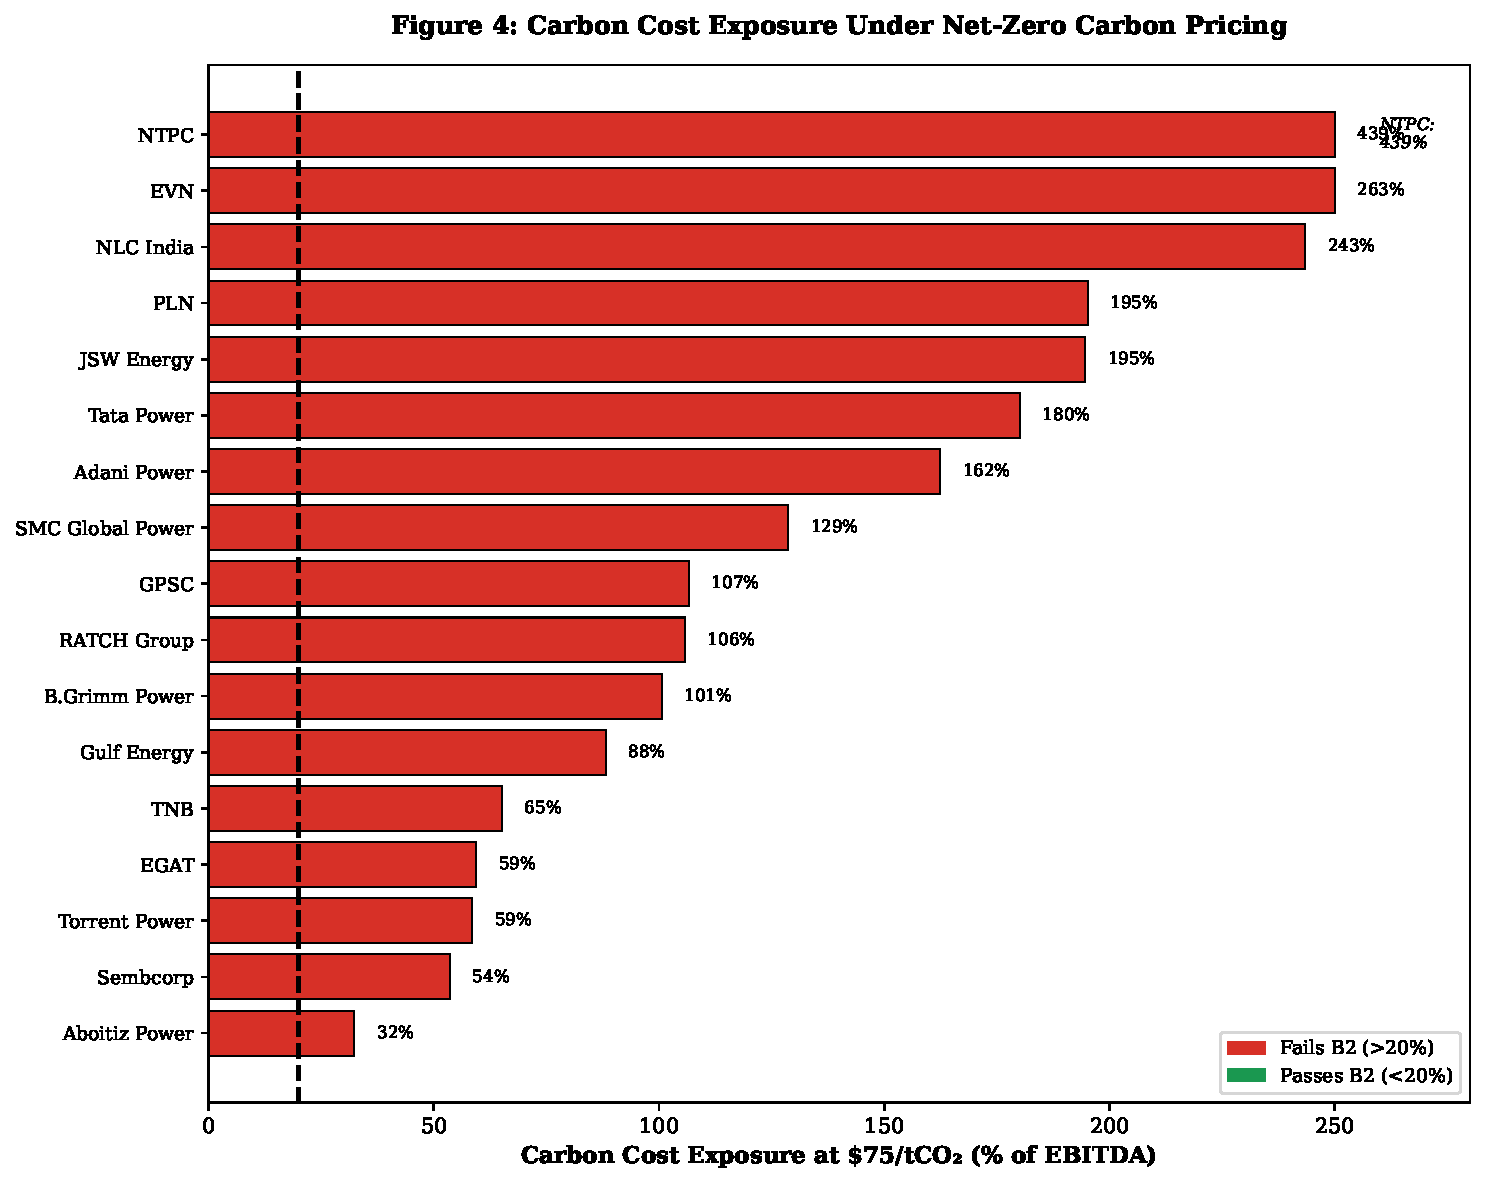
\includegraphics[width=\textwidth]{../figures/fig4_b2_sensitivity.pdf}
\caption{Carbon cost exposure as percentage of EBITDA at \$75/tCO$_2$ (Paris-aligned scenario). Red bars: exposure $>$ 20\% of EBITDA; green bars: $\leq$ 20\%. Dashed line marks 20\% threshold. Under current policy, most utilities face zero carbon cost.}
\label{fig:b2_sensitivity}
\end{figure}

% --- Financial constraints ---
\subsection{The Financial Trap: Coal Drag Constrains the Transition}
\label{sec:results_financial}

The generation gap shows that capacity additions alone do not displace coal. The missing carbon price shows that the market does not correct for this. A third constraint operates at the balance sheet level: even utilities that want to scale clean investment face financial limits that coal itself imposes. Six of fourteen coal-owning utilities face medium or high coal drag (Table~\ref{tab:coal_drag}).

\begin{table}[H]
\centering
\caption{Coal Drag Assessment (Coal-Owning Utilities)}
\label{tab:coal_drag}
\small
\begin{adjustbox}{max width=\linewidth}
\begin{tabular}{@{}llccccl@{}}
\toprule
\textbf{Utility} & \textbf{Country} & \textbf{Coal\%Gen} & \textbf{Debt/EBITDA} & \textbf{Clean CapEx\%} & \textbf{Score} & \textbf{Coal Drag} \\
\midrule
PLN & ID & 66\% & 5.3x & 15\% & 3/3 & High \\
SMC Global Power & PH & 78\% & 5.3x & -- & 2/3 & High \\
NTPC & IN & 87\% & 4.6x & 60\% & 2/3 & Medium \\
Tata Power & IN & 78\% & 4.3x & 55\% & 2/3 & Medium \\
JSW Energy & IN & 74\% & 8.1x & 75\% & 2/3 & Medium \\
EVN & VN & 70\% & 4.6x & 15\% & 2/3 & Medium \\
Adani Power & IN & 100\% & 1.2x & -- & 1/3 & Low \\
TNB & MY & 51\% & 2.9x & -- & 1/3 & Low \\
Aboitiz Power & PH & 72\% & 3.3x & 25\% & 1/3 & Low \\
NLC India & IN & 76\% & 3.4x & -- & 1/3 & Low \\
GPSC & TH & 17\% & 6.3x & -- & 1/3 & Low \\
RATCH Group & TH & 12\% & 5.4x & -- & 1/3 & Low \\
EGAT & TH & 20\% & 1.9x & -- & 0/3 & None \\
Torrent Power & IN & 10\% & 1.7x & 50\% & 0/3 & None \\
\bottomrule
\end{tabular}
\end{adjustbox}
\begin{flushleft}
\footnotesize{Coal\%Gen = coal share of estimated generation. Score components: (1) coal $>$50\% of generation, (2) Debt/EBITDA $\geq$ 4.0x, (3) clean CapEx $<$ 30\%. ``--'' indicates clean CapEx data not publicly disclosed; scored conservatively as failing unless other evidence suggests otherwise.}
\end{flushleft}
\end{table}

The double bind is clearest at PLN (High drag: 66\% coal generation, 5.3x leverage, 15\% clean CapEx) and NTPC (Medium drag: 87\% coal generation, 4.6x leverage, but 60\% clean CapEx). Even NTPC, with the highest clean CapEx share among major coal-owning utilities, cannot escape the constraint: its coal fleet generates the revenue to fund renewable expansion, but coal-related leverage leaves negative debt headroom ($-$0.6x below the 4.0x threshold), limiting how much more it can borrow.

A qualification: state-owned enterprises (NTPC, PLN, EVN) benefit from implicit sovereign guarantees that may soften the leverage constraint. Coal revenue dependency and insufficient clean CapEx still apply, but sovereign-backed access to concessional lending means the Debt/EBITDA threshold may overstate financial pressure for these utilities.

The timeline compounds the problem. At current deployment pace, matching coal generation in TWh would require multiplying aggregate renewable capacity 12.2 times, taking decades during which coal continues running.


% --- 5. Heterogeneity: Diagnostic results and business model ---
\subsection{Variation: Diagnostic Results by Business Model and Ownership}
\label{sec:results_ratings}

The previous three subsections established the generation gap, the missing carbon price, and coal drag as separate constraints. The full five-dimension diagnostic brings them together for each utility (Table~\ref{tab:results}). The pattern is clear: D2 and D3 pass for every utility (reflecting the absent carbon price), while D1 fails for every coal-owning utility (no retirement plans). D4 and D5 split the sample: five coal-owning utilities pass D4 (sufficient capital reallocation on paper), but none passes D1, meaning even utilities investing in renewables are not closing coal. The binding constraints are structural (no retirement pathways) and policy-driven (no carbon price), not technological.

\begin{table}[H]
\centering
\caption{Diagnostic Results by Utility. D1 = coal retirement pathways; D2 = carbon cost exposure; D3 = technology displacement; D4 = capital reallocation; D5 = balance sheet resilience.}
\label{tab:results}
\small
\begin{adjustbox}{max width=\linewidth}
\begin{tabular}{@{}llcccccr@{}}
\toprule
\textbf{Utility} & \textbf{Country} & \textbf{D1} & \textbf{D2} & \textbf{D3} & \textbf{D4} & \textbf{D5} & \textbf{Dims Met} \\
\midrule
Sembcorp & SG & \checkmark & \checkmark & \checkmark & \checkmark & $\times$ & 4/5 \\
Adani Green & IN & \checkmark & \checkmark & \checkmark & \checkmark & $\times$ & 4/5 \\
NHPC & IN & \checkmark & \checkmark & \checkmark & \checkmark & $\times$ & 4/5 \\
SJVN & IN & \checkmark & \checkmark & \checkmark & \checkmark & $\times$ & 4/5 \\
Gulf Energy & TH & \checkmark & \checkmark & \checkmark & \checkmark & $\times$ & 4/5 \\
B.Grimm Power & TH & \checkmark & \checkmark & \checkmark & \checkmark & $\times$ & 4/5 \\
Adani Power & IN & $\times$ & \checkmark & \checkmark & $\times$ & \checkmark & 3/5 \\
Torrent Power & IN & $\times$ & \checkmark & \checkmark & $\times$ & \checkmark & 3/5 \\
TNB & MY & $\times$ & \checkmark & \checkmark & $\times$ & \checkmark & 3/5 \\
EGAT & TH & $\times$ & \checkmark & \checkmark & $\times$ & \checkmark & 3/5 \\
EVN & VN & $\times$ & \checkmark & \checkmark & \checkmark & $\times$ & 3/5 \\
Tata Power & IN & $\times$ & \checkmark & \checkmark & \checkmark & $\times$ & 3/5 \\
JSW Energy & IN & $\times$ & \checkmark & \checkmark & \checkmark & $\times$ & 3/5 \\
NLC India & IN & $\times$ & \checkmark & \checkmark & $\times$ & \checkmark & 3/5 \\
Aboitiz Power & PH & $\times$ & \checkmark & \checkmark & \checkmark & \checkmark & 4/5 \\
NTPC & IN & $\times$ & \checkmark & \checkmark & \checkmark & $\times$ & 3/5 \\
PLN & ID & $\times$ & \checkmark & \checkmark & $\times$ & $\times$ & 2/5 \\
SMC Global Power & PH & $\times$ & \checkmark & \checkmark & $\times$ & $\times$ & 2/5 \\
GPSC & TH & $\times$ & \checkmark & \checkmark & $\times$ & $\times$ & 2/5 \\
RATCH Group & TH & $\times$ & \checkmark & \checkmark & $\times$ & $\times$ & 2/5 \\
\bottomrule
\end{tabular}
\end{adjustbox}
\begin{flushleft}
\footnotesize{D2 and D3 pass universally under current-policy prices because six of seven markets impose zero effective carbon price on power generation (Table~\ref{tab:carbon_prices}); these dimensions activate under forward scenarios (Table~\ref{tab:scenarios_new}). Six of the seven utilities scoring 4/5 fail D5, predominantly due to project-finance capital structures that inflate leverage metrics; Aboitiz Power (4/5) passes D5.}
\end{flushleft}
\end{table}


\begin{figure}[H]
\centering
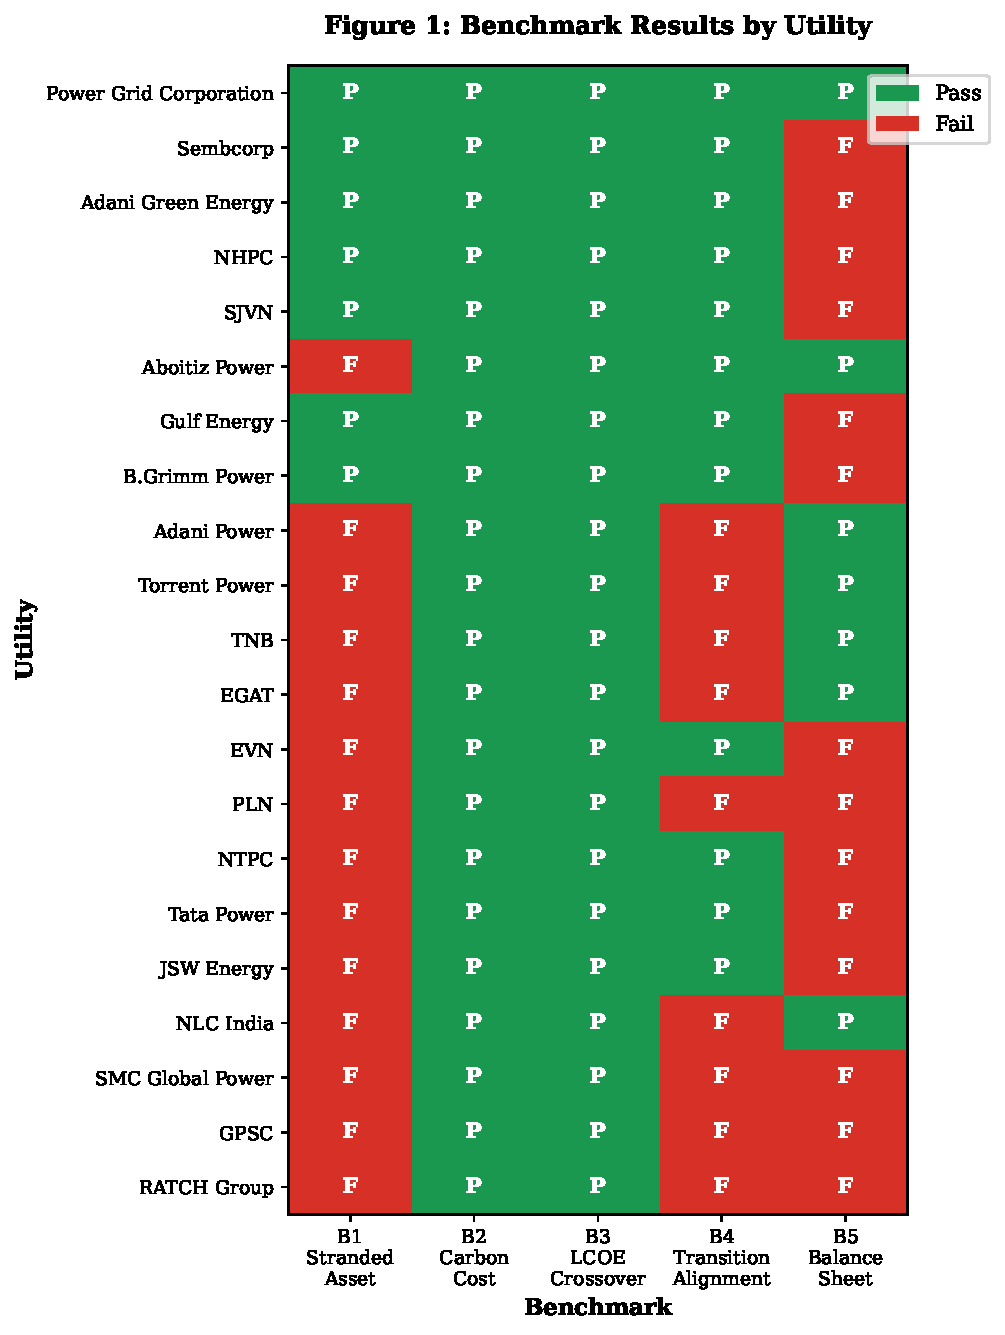
\includegraphics[width=\textwidth]{../figures/fig1_benchmark_heatmap.pdf}
\caption{Diagnostic heatmap by utility and dimension. Green = pass; red = fail. D2 and D3 pass universally under current carbon prices. D1 (coal retirement) fails for all coal-owning utilities.}
\label{fig:heatmap}
\end{figure}

Grow-out viability tracks business model, not ownership (Table~\ref{tab:ownership}). Pure-play renewable developers average 4.0 of 5 dimensions met; state-owned coal generators average 2.8. But this comparison is misleading: pure-play developers are not ``better at grow-out''; they are the \textit{alternative} to grow-out because they have no coal to grow out of. The relevant comparison is among coal-owning utilities, where what a utility owns (portfolio composition) matters more than who owns it (governance structure). The Adani Green versus Adani Power comparison illustrates this under shared governance: same conglomerate, opposite diagnostic profiles (4/5 versus 3/5), because the portfolio, not corporate strategy, determines the score.

\begin{table}[H]
\centering
\caption{Grow-Out Viability by Ownership and Business Model}
\label{tab:ownership}
\begin{adjustbox}{max width=\linewidth}
\begin{tabular}{@{}lcccc@{}}
\toprule
\textbf{Category} & \textbf{n} & \textbf{Avg Clean CapEx} & \textbf{Avg D1 Pass} & \textbf{Avg Dims Met} \\
\midrule
Pure-play RE & 4 & 85\% & 100\% & 4.0/5 \\
Private (diversified) & 8 & 59\% & 25\% & 3.0/5 \\
State-linked & 4 & 39\% & 0\% & 2.3/5 \\
State-owned & 4 & 50\% & 0\% & 2.8/5 \\
\bottomrule
\end{tabular}
\end{adjustbox}
\begin{flushleft}
\footnotesize{Averages computed across all 20 generation utilities.}
\end{flushleft}
\end{table}



If the diagnostic captures something real about grow-out viability, it should diverge from existing sustainability ratings, which measure disclosure and commitment rather than generation outcomes. It does. ESG environmental scores do not track grow-out viability (Table~\ref{tab:ratings}): Adani Green (ESG Env 86.5, 4/5 dimensions) outscores NTPC (67.9, 3/5), but Sembcorp (43.8, 4/5) scores lower than both. WBA ACT ratings add little discrimination, and SBTi has zero coverage. Ten of twenty utilities lack any external rating. Plant-level data from public registries remain the only consistent basis for assessing whether grow-out delivers emissions reductions.

\begin{table}[H]
\centering
\caption{External Ratings versus Diagnostic Assessment}
\label{tab:ratings}
\small
\begin{adjustbox}{max width=\linewidth}
\begin{tabular}{@{}llcccc@{}}
\toprule
\textbf{Utility} & \textbf{Country} & \textbf{ESG Env} & \textbf{WBA ACT} & \textbf{SBTi} & \textbf{Dims Met} \\
\midrule
Adani Green       & IN & 86.5 & --    & No & 4/5 \\
NTPC              & IN & 67.9 & 4/60  & No & 3/5 \\
Tata Power        & IN & 63.1 & 14/60 & No & 3/5 \\
TNB               & MY & 59.3 & 15/60 & No & 3/5 \\
RATCH Group       & TH & 57.0 & --    & No & 2/5 \\
Sembcorp          & SG & 43.8 & --    & No & 4/5 \\
SJVN              & IN & 38.8 & --    & No & 4/5 \\
NHPC              & IN & 34.4 & --    & No & 4/5 \\
Aboitiz Power     & PH & 26.6 & 13/60 & No & 4/5 \\
EVN               & VN & --   & 2/60  & No & 3/5 \\
\bottomrule
\end{tabular}
\end{adjustbox}
\begin{flushleft}
\footnotesize{ESG Env: Refinitiv environmental pillar score (0--100). WBA ACT: ACT subscale from the WBA Electric Utilities Benchmark 2023 (0--60) \citep{WBA2024}. SBTi: validated near-term target status (January 2026). ``--'' = no coverage. Remaining 10 utilities lack coverage on all three external ratings.}
\end{flushleft}
\end{table}

% --- 7. Robustness ---
\subsection{Robustness: Does Demand Growth Change the Result?}
\label{sec:robustness}

The results so far rest on a static assumption: coal running rates stay at 55\%. The most important objection to the baseline analysis is that adding renewables should push coal running rates down as cheaper power enters the grid. We test this by modelling coal as a residual supplier: coal fills whatever demand remains after renewables and gas have dispatched. Running rates adjust year by year depending on the balance between electricity demand, renewable deployment, and gas generation.

For each coal-owning utility, we project over 2025--2035:
\begin{equation}
D(t) = D_0 \times (1 + g)^t, \qquad RE_{MW}(t) = RE_{MW,0} + r \times t
\end{equation}
\noindent where $D(t)$ is electricity demand, $g$ is the country-specific annual demand growth rate, and $r$ is the annual renewable deployment rate from declared utility pipelines. Coal fills the residual:
\begin{equation}
CF_{coal}(t) = \text{clamp}\!\left(0.40,\; 0.70,\; \frac{D(t) - G_{RE}(t) - G_{gas}}{MW_{coal} \times 8{,}760}\right)
\end{equation}
\noindent The floor of 40\% represents minimum stable generation; the ceiling of 70\% represents the operational upper bound. Country-specific demand growth rates are from IEA World Energy Outlook 2024 and national planning documents: India 6.5\%, Vietnam 7\%, Indonesia 5\%, Philippines 5\%, Malaysia 3\%, Thailand 3\%, Singapore 1.5\%.

\begin{table}[H]
\centering
\caption{Dynamic Grow-Out Scenarios: Aggregate Coal Emissions (14 Coal-Owning Utilities, 2025--2035)}
\label{tab:dynamic}
\small
\begin{adjustbox}{max width=\linewidth}
\begin{tabular}{@{}llccrr@{}}
\toprule
\textbf{Scenario} & \textbf{Demand growth} & \textbf{RE deployment} & \textbf{Coal CF} & \textbf{2035 MtCO$_2$} & \textbf{$\Delta$ vs 2025} \\
\midrule
A: Baseline & Country rates (5--7\%) & Actual pipeline & Dynamic & 858 & $+$2.8\% \\
B: Moderate & Country $-$2pp (3--5\%) & Pipeline $\times$1.5 & Dynamic & 857 & $+$2.7\% \\
C: Optimistic & Country $-$3pp (2--4\%) & Pipeline $\times$2 & Dynamic & 741 & $-$11.2\% \\
D: Zero growth & 0\% & Pipeline $\times$2 & Dynamic & 655 & $-$21.5\% \\
\midrule
\textit{Static baseline} & \textit{n/a} & \textit{n/a} & \textit{Fixed 55\%} & \textit{706} & \textit{n/a} \\
\bottomrule
\end{tabular}
\end{adjustbox}
\begin{flushleft}
\footnotesize{Coal CF bounded by [40\%, 70\%]. RE blended CF = 22\%. Gas CF = 50\% (fixed). Emission factor = 0.91~tCO$_2$/MWh. RE deployment rates from utility pipeline disclosures. 2025 base emissions (834~MtCO$_2$) exceed the static estimate (706~MtCO$_2$) because several utilities already run above 55\%. Full utility-level results in Appendix~\ref{app:dynamic}.}
\end{flushleft}
\end{table}

The dynamic analysis strengthens rather than weakens the baseline finding. Under realistic demand growth (Scenarios~A and~B), total coal emissions \textit{increase} by roughly 3\%, because rising consumption absorbs new renewable output before it can displace coal. In Scenario~A, 100\% of new renewable generation is absorbed by demand growth for 10 of 14 utilities. Coal running rates rise toward the 70\% ceiling, confirming that the static 55\% assumption is conservative, not aggressive. Even under optimistic assumptions (Scenario~C: halved demand growth, doubled renewable deployment), emissions fall by only 11\%, insufficient for Paris-aligned trajectories and contingent on assumptions well beyond current plans. Only under zero demand growth (Scenario~D) do renewables produce a large reduction ($-$21.5\%), a scenario with no basis in current projections for these markets.

The dynamic analysis also reveals a further risk: in coal-heavy grids with inflexible dispatch, rising renewable capacity alongside rigid coal operations can lead to curtailment of renewable generation, meaning the grow-out strategy may strand renewable investment as well as fail to reduce emissions. Vietnam's grid already experiences 10--30\% curtailment in solar-rich provinces due to transmission constraints and inflexible coal dispatch.

% --- 8. Synthesis ---
\subsection{Summary of Findings}

The results establish three facts. First, the generation gap: renewable capacity additions do not translate proportionally into generation displacement because coal plants produce far more electricity per megawatt than solar or wind. Second, the missing market correction: the absence of carbon pricing in six of seven markets removes the signal that could force coal off the grid, and regulated market structures prevent cheaper renewables from displacing coal through competition. Third, the financial trap: coal provides the revenue that funds the transition while simultaneously constraining the borrowing needed to scale it. These three constraints reinforce each other: the generation gap means grow-out requires massive renewable scaling, the missing carbon price means there is no market pressure to retire coal, and coal drag means utilities lack the financial capacity to build renewables fast enough. Under dynamic demand growth, the picture worsens: emissions increase rather than decline. The grow-out strategy expands the energy system but does not reduce coal emissions at the firm level.

%% ============================================================
%% 5. DISCUSSION
%% ============================================================
\section{Discussion}
\label{sec:discussion}

\subsection{Why Grow-Out Fails and What Would Fix It}

Grow-out fails as climate policy not because adding renewables is wrong, but because adding renewables alone is insufficient in markets where coal has guaranteed dispatch, demand is growing, and no carbon price forces a change in the generation mix. The capacity factor wedge ensures that MW additions translate into far less TWh displacement than headline figures suggest; demand growth absorbs what displacement does occur; and coal drag limits the financial capacity to accelerate deployment. The strategy succeeds as energy policy precisely because it expands the system without disrupting the political and contractual structures around coal.

This interpretation helps reconcile conflicting signals in the literature. \citet{York2012} found that non-fossil energy displaces less than one-quarter of fossil energy globally, a finding often attributed to political economy or lock-in. Our firm-level data suggests a more specific mechanism: in high-growth Asian markets, the displacement coefficient is low mainly because demand growth absorbs new renewable output before it reaches coal. This is not lock-in in the institutional sense \citep{Alova2020}; it is a direct consequence of the capacity factor gap. The capacity factor wedge and demand absorption together explain why three-quarters of utilities worldwide have not meaningfully shifted portfolios over two decades, without requiring appeal to political resistance as the primary cause.

The coal drag construct integrates what the literature has documented separately. \citet{Ameli2021} formalised a climate investment trap at the country level; \citet{Kungl2018} documented structural destabilisation of European incumbents; \citet{CarbonTracker2021} quantified stranded-asset exposure. Coal drag operates at the firm level, capturing a paradox none of these frameworks addresses individually: coal generates the cash flow funding renewable expansion while simultaneously constraining the balance sheet to scale it. The six utilities in our sample facing medium or high coal drag are not failing to transition because of insufficient ambition; they are constrained by the financial structure of their own portfolios.

\subsection{Four Mechanisms to Make Grow-Out Work}

If the diagnosis is correct, the prescription follows directly. Each of the four binding constraints maps to a specific mechanism that can be implemented without requiring plant closure.

\textit{Dispatch reform} is the lowest-hanging intervention. China's equal-share dispatch system produced an additional 3~GtCO$_2$ over 2011--2019 \citep{Yu2023}. India's SCED pilot, covering 56~GW, achieved cumulative savings of \$260~million between 2019 and 2022. In a merit-order system, high-cost coal plants lose dispatch hours to cheaper alternatives without requiring closure. In PPA-dominated markets, dispatch reform requires regulatory restructuring of minimum offtake guarantees.

\textit{PPA renegotiation} unlocks the contractual bottleneck. Over 90\% of coal capacity in our sample operates under take-or-pay contracts with guaranteed dispatch \citep{Boute2025}. The practical pathway is modification rather than termination: reducing minimum offtake, remunerating flexibility services, and replacing coal PPAs with clean energy PPAs at renegotiation windows. Financial modelling of Indonesian PPAs suggests 80--90\% emissions reductions while maintaining investor returns \citep{Bodnar2020}.

\textit{Managed capacity factor decline} repositions coal from baseload to balancing. Committed emissions are directly sensitive to utilisation rates \citep{Tong2019}. China's 360~GW flexibility retrofit programme demonstrates that repositioning coal to flexible dispatch saves \$176~billion versus early retirement while allowing integration of 194--245~GW of additional renewables \citep{An2025}. Reducing coal CFs from 55\% to 40\% in our sample would cut aggregate emissions by approximately 27\% without closing a single plant.

\textit{Solar-plus-storage} closes the capacity factor wedge. Storage converts intermittent solar (20\% CF) into firm power ($>$90\% availability), letting renewables compete for coal's dispatch hours. Indian auction results show solar-plus-storage at \$0.036--0.041/kWh, approaching new coal parity at \$0.065--0.071/kWh.

These mechanisms form a natural policy sequence: dispatch reform creates the economic pressure that makes PPA renegotiation rational; PPA restructuring opens the door to managed PLF decline without triggering buyout costs; flexibilisation repositions coal as a balancing resource; and storage progressively captures its remaining hours. Each has been demonstrated in at least one Asian context, and each preserves plant operation while reducing generation, aligning with the political objectives that dominate energy policy in these markets \citep{Ohlendorf2022}.

Carbon pricing should, in principle, provide the market signal that makes these mechanisms unnecessary. Our finding that six of seven markets impose zero or negligible carbon prices explains why it does not. The structural barrier runs deeper than the price level: the regulated tariffs and PPAs that insulate coal from market signals would equally insulate it from carbon prices unless pass-through is prohibited, a condition no market in our sample has imposed \citep{Boute2017,Acworth2020}. The four mechanisms function as substitutes for the absent price signal.

\subsection{Implications for Credibility Assessment and Transition Finance}

The four mechanisms address what utilities and regulators can do differently. A separate question is what investors, rating agencies, and multilateral institutions should measure differently. The capacity factor wedge has direct implications for how transition progress is assessed. Every utility in our sample has renewable capacity targets; the diagnostic shows these translate into far less generation displacement than MW figures suggest. Three consequences follow.

First, transition plan credibility requires MW-to-TWh conversion. Any assessment framework that evaluates utilities on planned capacity additions without applying fuel-specific capacity factors will overstate progress. ESG environmental scores diverge from grow-out viability, WBA ACT ratings add limited discrimination, and SBTi has zero coverage in our sample. Plant-level registries such as the Global Energy Monitor, which track unit status and capacity factors quarterly, provide a more reliable basis for assessing coal transition than any corporate-level rating \citep{Duchin2025,Jiang2025,Berg2022}.

Second, national targets embed the same accounting gap. India's 500~GW non-fossil target and Indonesia's 42.6~GW RUPTL RE target both express ambition in MW. Our analysis shows that MW-denominated targets in high-demand-growth markets are consistent with zero emissions reduction. Credibility assessments of NDCs and JETP commitments should require TWh-denominated disclosure alongside MW targets, and demand-growth absorption analysis should be standard in monitoring frameworks.

Third, transition finance products need to be structured around the four mechanisms, not around generic renewable deployment. Green bonds and transition bonds that finance renewable capacity for thermal incumbents without addressing dispatch, PPAs, or capacity factor management are vulnerable to the fungibility problem our data documents. Finance products structured around dispatch reform outcomes, PPA restructuring milestones, verified capacity factor decline trajectories, or storage-backed coal displacement have clearer additionality. The coal drag diagnostic provides a screening tool for identifying which utilities can absorb transition finance productively and which will add RE alongside unchanged coal operation.

\subsection{Scope and Limitations}

The analysis identifies what prevents grow-out from working and what could make it work. A natural question is where these findings apply. The results hold most directly in regulated Asian electricity markets with high demand growth, young coal fleets, and PPA-dominated dispatch. In liberalised markets with flat demand and merit-order dispatch (Europe, parts of the US), the grow-out calculation may close differently because the mechanisms we identify as absent are already present. The diagnostic framework is designed to test this.

Three methodological limitations warrant acknowledgment. First, the dynamic model treats coal as a residual supplier in a simplified dispatch framework; real-world dispatch involves unit commitment constraints, ramping costs, and minimum run times. Second, the diagnostic evaluates technology displacement through standalone LCOE, which does not capture integration costs, curtailment risks, or grid constraints. Third, BESS cost trajectories could reshape the grow-out calculus: if storage enables renewables to compete for baseload dispatch hours, coal PLFs would decline even with demand growth. Indian solar-plus-storage costs are approaching new coal parity but remain above existing coal variable cost (\$35/MWh) and are not yet competitive in Vietnam (\$167/MWh) or the Philippines (\$94/MWh).

The finding itself is narrower than ``grow-out is wrong'': it is that grow-out as currently practised does not reduce absolute emissions. With the four complementary mechanisms, grow-out could work as climate policy. The sample covers seven markets and 20 utilities; generalisability to other regions remains an open question.

Future research should model the compound effects of all four mechanisms on coal generation trajectories for specific utilities, quantify the financial costs of PPA restructuring versus continued coal operation, and examine how dispatch reform interacts with emerging carbon pricing in regulated Asian markets.

%% ============================================================
%% 6. CONCLUSIONS
%% ============================================================
\section{Conclusion}
\label{sec:conclusion}

% --- Core takeaway ---
The ``grow out of coal'' strategy rests on a unit conversion error. A megawatt of coal generates roughly 2--3 times the annual electricity of a megawatt of solar or wind, so adding renewable capacity alongside an operating coal fleet reduces coal's share of the mix without reducing coal's contribution to the atmosphere. Across 20 utilities and 310~GW in emerging Asia, this paper shows that the strategy succeeds as energy policy and fails as climate policy, not because of political resistance or institutional lock-in, but because of the capacity factor gap between coal and renewables.

% --- Re-answer the research question ---
We asked whether grow-out produces measurable reductions in total coal generation and emissions at the firm level. The answer is that it does not. Renewables account for 12.5\% of installed capacity but only 5.7\% of generation. Even doubling every utility's renewable capacity, coal still supplies 67\% of electricity. Under demand growth of 5--7\% per year, emissions increase rather than decline, because new renewable output is absorbed by rising consumption before it reaches coal. Six of seven markets charge nothing for carbon emissions, removing the only price signal that could change the dispatch order.

% --- Contribution ---
The paper establishes three results that the existing literature has not. First, it quantifies the capacity factor wedge at the firm level, showing precisely how MW additions fail to translate into TWh displacement for individual utilities. Second, it introduces coal drag as a financial mechanism: coal simultaneously funds and constrains the transition, trapping six of fourteen thermal incumbents in a portfolio structure that limits the borrowing capacity needed to scale renewable investment. Third, it brings the concept of aid fungibility into transition finance, demonstrating that financial support channelled through coal-owning utilities can be absorbed without producing coal retirement.

% --- Broader implications ---
These findings extend beyond emerging Asia. Any electricity system where coal operates under long-term contracts with guaranteed dispatch, where demand is growing, and where no carbon price forces a change in the generation mix faces the same problem. The diagnostic framework requires only publicly available capacity data and fuel-specific running rates; it can be applied to any utility, in any market, to test whether the grow-out calculation closes. The wider point is that transition progress measured in MW is structurally misleading wherever a capacity factor gap exists between the technology being added and the technology it is supposed to replace.

% --- Policy message ---
The policy takeaway is specific: transition plans, national targets, and JETP commitments expressed in MW should be accompanied by TWh-denominated disclosure, and transition finance should be conditioned on the mechanisms that actually reduce coal generation. Dispatch reform, PPA renegotiation, managed capacity factor decline, and solar-plus-storage deployment form a natural sequence, each demonstrated in at least one Asian context, that can make grow-out work without requiring plant closure. Finance products structured around these mechanisms have clear additionality; those structured around generic renewable deployment do not.

% --- Forward-looking insight ---
Whether cheaper storage, emerging carbon markets, or slowing demand growth will eventually close the grow-out gap for specific utilities is an empirical question the framework is designed to answer. What the current data show is that the gap is not closing on its own.

\section*{CRediT authorship contribution statement}

\textbf{Jose Luis Resendiz:} Conceptualization, Methodology, Formal analysis, Investigation, Data curation, Writing (original draft), Writing (review \& editing), Visualization. \textbf{Gireesh Shrimali:} Supervision, Writing (review \& editing).

\section*{Declaration of competing interest}

The authors declare that they have no known competing financial interests or personal relationships that could have appeared to influence the work reported in this paper.

\section*{Data availability}

The Asian Utilities Transition Database supporting this analysis will be deposited in the Oxford University Research Archive (ORA) upon acceptance. The replication package includes utility-level inputs, diagnostic calculations, source documentation, and code. Until deposit, the dataset is available from the corresponding author upon reasonable request.

\section*{Acknowledgments}

The authors thank colleagues at the Smith School of Enterprise and the Environment for helpful comments. Any remaining errors are our own.

\section*{Funding}

This research did not receive any specific grant from funding agencies in the public, commercial, or not-for-profit sectors.

%% ============================================================
%% APPENDICES
%% ============================================================
\appendix

\section{Full Grow-Out Generation Accounting Table}
\label{app:growout_full}

\begin{table}[H]
\centering
\caption{Grow-Out Generation Accounting: All Thermal Incumbents and Pure-Play RE Developers. Coal CF = 55\%; Solar CF = 20\%; Wind CF = 30\%. Emission factor = 0.91~tCO$_2$/MWh.}
\label{tab:growout_full}
\small
\begin{adjustbox}{max width=\linewidth}
\begin{tabular}{@{}llrrrrrrl@{}}
\toprule
\textbf{Utility} & \textbf{Country} & \textbf{Coal MW} & \textbf{RE MW} & \textbf{Coal TWh} & \textbf{RE TWh} & \textbf{Coal\%} & \textbf{RE/Coal} & \textbf{Coal MtCO$_2$} \\
\midrule
NTPC & IN & 65,194 & 10,175 & 314.1 & 18.7 & 87\% & 0.06 & 285.8 \\
PLN & ID & 35,000 & 476 & 168.6 & 1.0 & 66\% & 0.01 & 153.5 \\
Adani Power & IN & 15,210 & 40 & 73.3 & 0.1 & 100\% & 0.00 & 66.7 \\
EVN & VN & 12,678 & 2,000 & 61.1 & 3.9 & 70\% & 0.07 & 55.6 \\
Tata Power & IN & 7,800 & 5,220 & 37.6 & 10.1 & 78\% & 0.27 & 34.2 \\
TNB & MY & 6,810 & 1,304 & 32.8 & 2.5 & 51\% & 0.07 & 29.9 \\
JSW Energy & IN & 5,658 & 3,826 & 27.3 & 9.5 & 74\% & 0.35 & 24.8 \\
SMC Global Power & PH & 3,756 & -- & 18.1 & -- & 78\% & 0.00 & 16.5 \\
Aboitiz Power & PH & 3,073 & 252 & 14.8 & 0.4 & 72\% & 0.03 & 13.5 \\
EGAT & TH & 2,220 & 106 & 10.7 & 0.2 & 22\% & 0.02 & 9.7 \\
NLC India & IN & 1,660 & 1,431 & 8.0 & 2.6 & 76\% & 0.32 & 7.3 \\
GPSC & TH & 900 & 4,667 & 4.3 & 8.3 & 17\% & 1.92 & 3.9 \\
RATCH Group & TH & 742 & 905 & 3.6 & 2.3 & 12\% & 0.65 & 3.3 \\
Torrent Power & IN & 362 & 1,746 & 1.7 & 3.9 & 10\% & 2.22 & 1.6 \\
\midrule
\textit{Aggregate} & & \textit{161,063} & \textit{32,148} & \textit{776.0} & \textit{63.5} & \textit{71\%} & \textit{0.08} & \textit{706.3} \\
\midrule
\multicolumn{9}{l}{\textit{Non-coal utilities (no coal to grow out of):}} \\
Adani Green & IN & -- & 15,816 & -- & 29.9 & -- & -- & -- \\
Sembcorp$^{\dagger}$ & SG & -- & 15,549 & -- & 33.8 & -- & -- & -- \\
SJVN & IN & -- & 1,174 & -- & 2.1 & -- & -- & -- \\
B.Grimm Power & TH & -- & 1,073 & -- & 1.9 & -- & -- & -- \\
Gulf Energy & TH & -- & 1,064 & -- & 2.5 & -- & -- & -- \\
NHPC & IN & -- & 561 & -- & 1.0 & -- & -- & -- \\
\bottomrule
\end{tabular}
\end{adjustbox}
\begin{flushleft}
\footnotesize{Coal\% = coal share of estimated generation (coal + gas + RE). RE/Coal = ratio of RE generation to coal generation. RE MW excludes hydro for comparability. Gas capacity (59,279~MW aggregate) produces 259.8~TWh but is omitted for clarity; included in Coal\% denominator. TNB capacity includes equity stakes in IPP projects (consolidated boundary). Sembcorp gross portfolio includes projects under development; operational capacity is lower. $^{\dagger}$Sembcorp has significant gas capacity (and non-zero carbon cost exposure under Singapore's carbon tax) but no coal; classified as non-coal rather than pure-play RE.}
\end{flushleft}
\end{table}

\section{Full Carbon Cost Exposure Table}
\label{app:carbon_full}

\begin{table}[H]
\centering
\caption{Carbon Cost Exposure by Carbon Price Scenario, All Utilities with Fossil Generation (\% of EBITDA)}
\label{tab:scenarios_full}
\begin{adjustbox}{max width=\linewidth}
\begin{tabular}{@{}llccc@{}}
\toprule
\textbf{Utility} & \textbf{Country} & \textbf{Current policy} & \textbf{\$15 floor} & \textbf{\$75 stress} \\
\midrule
NTPC & IN & 0.0\%$^{*}$ & 87.8\% & 439.0\% \\
EVN & VN & 0.0\%$^{*}$ & 52.6\% & 263.0\% \\
NLC India & IN & 0.0\%$^{*}$ & 48.7\% & 243.4\% \\
PLN & ID & 10.4\%$^{\dagger}$ & 39.0\% & 195.2\% \\
JSW Energy & IN & 0.0\%$^{*}$ & 38.9\% & 194.6\% \\
Tata Power & IN & 0.0\%$^{*}$ & 36.0\% & 180.1\% \\
Adani Power & IN & 0.0\%$^{*}$ & 32.5\% & 162.4\% \\
SMC Global Power & PH & 0.0\%$^{*}$ & 25.7\% & 128.7\% \\
GPSC & TH & 0.0\%$^{*}$ & 21.3\% & 106.6\% \\
RATCH Group & TH & 0.0\%$^{*}$ & 21.1\% & 105.7\% \\
B.Grimm Power & TH & 0.0\%$^{*}$ & 20.1\% & 100.6\% \\
Gulf Energy & TH & 0.0\%$^{*}$ & 17.6\% & 88.1\% \\
TNB & MY & 0.0\%$^{*}$ & 13.0\% & 65.1\% \\
EGAT & TH & 0.0\%$^{*}$ & 11.9\% & 59.4\% \\
Torrent Power & IN & 0.0\%$^{*}$ & 11.7\% & 58.5\% \\
Sembcorp & SG & 13.9\%$^{\ddagger}$ & 10.7\% & 53.6\% \\
Aboitiz Power & PH & 0.0\%$^{*}$ & 6.5\% & 32.4\% \\
\bottomrule
\end{tabular}
\end{adjustbox}
\begin{flushleft}
\footnotesize{$^{*}$Zero effective carbon price on power generation. $^{\dagger}$Indonesia \$4/tCO$_2$ (coal plants only). $^{\ddagger}$Singapore \$18.29/tCO$_2$ (all fossil fuels). Pure-play renewable utilities (Adani Green, NHPC, SJVN) omitted due to near-zero CCE. At \$75/tCO$_2$, sixteen of seventeen utilities exceed 50\% of EBITDA; all seventeen exceed 20\%.}
\end{flushleft}
\end{table}

\section{Methodological Details}
\label{app:methods}

This appendix provides additional detail on diagnostic criteria, including limitations acknowledged in the relevant literature and scenario parameters.

\subsection{Diagnostic Limitations}

Each dimension involves simplifications that warrant acknowledgment.

\textbf{D1 (Coal Retirement Pathways):} The capacity-based approach prioritises auditability over economic precision. NPV-based methods could yield different risk rankings, and undisclosed retirement dates may understate stranding risk \citep{CarbonTracker2018}. We treat the 20\% threshold as a conservative screen rather than a valuation.

\textbf{D2 (Carbon Cost Exposure):} We assume zero pass-through as a stress test. Pass-through varies widely by market design, so the 20\% threshold may be permissive for forward-looking credit assessment \citep{Sijm2006}.

\textbf{D3 (Technology Displacement Pressure):} LCOE comparisons omit integration costs and value factors at high renewable penetration \citep{Hirth2015,Hirth2013,IEATechno2024}. We interpret LCX as a first-order screen, not a dispatch model.

\textbf{D4 (Capital Reallocation):} The two-of-four rule guards against cheap-talk targets \citep{Rogelj2023}. The 30\% renewable-share threshold may be dated, and we document sub-criteria for each utility in the replication package.

\textbf{D5 (Balance Sheet Resilience):} The FFO/Debt threshold is conservative by design. Leverage and liquidity screens are heuristic IG conventions, and traditional credit metrics may miss long-term transition risk.

\subsection{Data Construction Details}
\label{app:data_considerations}

\subsubsection*{Harmonisation and Estimation Choices}

\begin{table}[htbp]
\centering
\caption{Data Harmonisation and Estimation Choices}
\label{tab:harmonisation}
\small
\begin{tabularx}{\textwidth}{lX}
\toprule
\textbf{Element} & \textbf{Approach} \\
\midrule
Currency and scale & All financial values converted to USD using year-end exchange rates for the reporting year; where fiscal years differ, we use the most recent available year and record vintage. \\
\addlinespace
Capacity taxonomy & Generation capacity mapped to a consistent technology taxonomy (coal, gas, hydro, solar, wind, other renewables), distinguishing equity/owned capacity from system capacity for vertically integrated utilities. \\
\addlinespace
Emissions estimation & Where Scope~1 emissions are not disclosed, we estimate emissions from portfolio generation by fuel (or, when unavailable, portfolio composition with standard utilisation assumptions) using IPCC default emission factors (coal: 0.91, gas: 0.40~tCO$_2$/MWh). Table~\ref{tab:emissions_validation} identifies which utilities rely on estimated versus reported data and compares our estimates against disclosed Scope~1 emissions where available. \\
\addlinespace
CapEx classification & Clean CapEx includes renewables, grids, storage, and other enabling investments; fossil expansion and material life-extension CapEx are treated as misaligned. Where technology-level CapEx is not disclosed, we triangulate using commissioned project additions, disclosed pipelines, and use-of-proceeds reporting. Table~\ref{tab:capex_criteria} provides the classification criteria and data sources for each utility. \\
\addlinespace
Credit metrics & Credit ratios computed from consolidated statements where possible and cross-checked against rating reports given differences in definitions (e.g., EBITDA versus FFO). \\
\bottomrule
\end{tabularx}
\end{table}

\subsubsection*{Carbon Pricing Jurisdiction Details (D2)}

Verified jurisdiction-level carbon prices and coverage are summarised in Table~\ref{tab:carbon_prices}. We document policy source checks and coverage assumptions in the replication package.

\subsubsection*{Data Considerations by Dimension}

Each dimension involves specific data challenges: D1 relies on plant-level retirement dates that most utilities do not disclose (we cross-validate against GEM and conservatively treat undisclosed capacity as at risk); D2 requires Scope~1 emissions often estimated from portfolio composition using IPCC emission factors \citep{IPCC2006} and assumes zero pass-through as an upper bound \citep{Sijm2006}; D3 uses IRENA/BNEF LCOE benchmarks interpreted as first-order screens rather than dispatch simulations \citep{Hirth2015}; D4 triangulates clean CapEx from project additions, pipelines, and use-of-proceeds reporting; D5 cross-checks credit metrics against rating reports to address variation in accounting standards and FFO definitions. Financial data vintage ranges from FY2023--2024 depending on reporting cycles. Full dimension-by-dimension data construction details, including source documentation and estimation choices for each utility, are provided in the replication package.

\subsection{Threshold Sensitivity}

To test whether diagnostic classifications hinge on precise threshold choices, we reclassify utilities under $\pm10\%$ shifts to the D1, D2, and D4 cutoffs. Classifications are unchanged: no utility changes tier under these perturbations (Table~\ref{tab:threshold_sensitivity}).

\begin{table}[H]
\centering
\caption{Diagnostic Stability Under $\pm10\%$ Threshold Shifts (D1, D2, D4)}
\label{tab:threshold_sensitivity}
\small
\begin{tabular}{@{}lccc@{}}
\toprule
\textbf{Dimensions passed} & \textbf{Baseline} & \textbf{Thresholds $-10\%$} & \textbf{Thresholds $+10\%$} \\
\midrule
5 of 5 & 0 & 0 & 0 \\
4 of 5 & 7 & 7 & 7 \\
3 of 5 & 9 & 9 & 9 \\
2 of 5 & 4 & 4 & 4 \\
1 of 5 & 0 & 0 & 0 \\
0 of 5 & 0 & 0 & 0 \\
\bottomrule
\end{tabular}
\begin{flushleft}
\footnotesize{Note: Thresholds shifted by $\pm10\%$ relative to baseline: D1 at-risk share 20\% $\rightarrow$ 18/22\%; D2 CCE/EBITDA 20\% $\rightarrow$ 18/22\%; D4 clean CapEx 50\% $\rightarrow$ 45/55\% and renewable share 30\% $\rightarrow$ 27/33\%. D4 retains the two-of-four rule. Carbon prices use verified January 2026 policy rates. All 20 generation utilities included.}
\end{flushleft}
\end{table}

\begin{table}[H]
\centering
\caption{Continuous Indicator Summary Statistics (D1, D3, D4, D5)}
\label{tab:continuous_summary}
\small
\begin{tabular}{@{}lcccc@{}}
\toprule
\textbf{Indicator} & \textbf{n} & \textbf{Min} & \textbf{Median} & \textbf{Max} \\
\midrule
D1 at-risk coal share (\%) & 20 & 0.0 & 85.4 & 100.0 \\
D3 displaced thermal share (\%) & 20 & 0.0 & 0.0 & 5.3 \\
D4 clean CapEx share (\%) & 13 & 15.0 & 67.0 & 100.0 \\
D5 credit metrics passed (0--5) & 20 & 0 & 3 & 5 \\
\bottomrule
\end{tabular}
\begin{flushleft}
\footnotesize{Note: Continuous indicators are drawn from the replication package. D1 and D3 are shares of capacity; D4 is clean CapEx share; D5 reports the number of credit metrics passed. D2 continuous CCE/EBITDA values are reported in Table~\ref{tab:scenarios_new}.}
\end{flushleft}
\end{table}

\subsection{Scenario Parameters}
\label{app:scenarios}

Table~\ref{tab:app_scenarios} details the scenario parameters used in the analysis.

\begin{table}[htbp]
\centering
\caption{Scenario Parameters}
\label{tab:app_scenarios}
\small
\begin{tabularx}{\textwidth}{llX}
\toprule
\multicolumn{3}{l}{\textbf{Panel A: Carbon Price Scenarios}} \\
\midrule
Scenario & Price & Rationale \\
\midrule
Current policy & \$0--18.29/tCO$_2$ & Verified country-specific prices on power generation: Singapore (\$18.29), Indonesia (\$4.00 coal only), India/Thailand/Vietnam/Philippines/Malaysia (\$0) \\
\$15 floor & \$15/tCO$_2$ & Near-term policy trajectory for most Asian markets \\
\$75 stress & \$75/tCO$_2$ & IEA Net Zero advanced-economy benchmark (used as Paris-aligned stress test) \citep{IEA2023} \\
\addlinespace
\midrule
\multicolumn{3}{l}{\textbf{Panel B: Solar-plus-Storage LCOE by Country}} \\
\midrule
Country & LCOE & Notes \\
\midrule
India & \$42/MWh & High irradiance and competitive auction outcomes \\
Indonesia & \$100/MWh & Estimated from solar PV mid + storage adder \\
Thailand & \$79/MWh & \\
Singapore & \$82/MWh & Land-constrained \\
Malaysia & \$83/MWh & \\
Philippines & \$94/MWh & \\
Vietnam & \$167/MWh & Grid integration challenges \\
\addlinespace
\midrule
\multicolumn{3}{l}{\textbf{Panel C: Thermal Generation Cost Assumptions}} \\
\midrule
Fuel & Base Cost & Carbon Intensity \\
\midrule
Coal & \$20/MWh & 0.91~tCO$_2$/MWh \\
Gas & \$35/MWh & 0.40~tCO$_2$/MWh \\
Oil & \$65/MWh & 0.78~tCO$_2$/MWh \\
\bottomrule
\end{tabularx}
\vspace{0.5em}
\noindent\small\textit{Note:} Variable costs for thermal generation equal base cost plus carbon cost (intensity $\times$ carbon price).
\end{table}

\subsection{Balance Sheet Resilience Metrics}
\label{app:b5metrics}

Table~\ref{tab:app_b5metrics} presents the credit metrics used for D5.

\begin{table}[htbp]
\centering
\caption{Balance Sheet Resilience Metrics}
\label{tab:app_b5metrics}
\begin{adjustbox}{max width=\linewidth}
\begin{tabular}{@{}lll@{}}
\toprule
\textbf{Metric} & \textbf{Pass Threshold} & \textbf{Rationale} \\
\midrule
\multicolumn{3}{l}{\textbf{Metrics with direct source}} \\
\midrule
Interest Coverage & $>$2.5x & Moody's utilities methodology \citep{Moodys2024} \\
FFO/Debt & $>$20\% & Moody's utilities methodology (conservative) \citep{Moodys2024} \\
\addlinespace
\multicolumn{3}{l}{\textbf{Heuristic IG screens informed by rating frameworks}} \\
\midrule
Debt/EBITDA & $<$4.0x & S\&P Corporate Methodology boundary between ``significant'' and ``aggressive'' financial risk profiles \citep{SPRatings2024} \\
Debt/Capital & $<$60\% & Fitch corporate criteria leverage conventions \citep{Fitch2024} \\
Current Ratio & $>$1.0x & Standard liquidity adequacy screen \\
\bottomrule
\end{tabular}
\end{adjustbox}
\end{table}

\section{Clean CapEx Classification Criteria}
\label{app:capex}

Table~\ref{tab:capex_criteria} documents the classification criteria, data sources, and assumptions used to compute the clean CapEx percentage for each utility where this metric is reported in the coal drag assessment.

\begin{table}[H]
\centering
\caption{Clean CapEx Classification by Utility}
\label{tab:capex_criteria}
\small
\begin{adjustbox}{max width=\linewidth}
\begin{tabular}{@{}llcl@{}}
\toprule
\textbf{Utility} & \textbf{Clean CapEx \%} & \textbf{Source type} & \textbf{Classification basis} \\
\midrule
NTPC & 60\% & Annual Report & RE segment CapEx (NGEL) / total consolidated CapEx \\
Tata Power & 55\% & Annual Report & Clean energy segment CapEx / total CapEx \\
JSW Energy & 75\% & Annual Report & RE project additions / total project additions \\
EVN & 15\% & Estimated & RE commissioned MW value / total commissioned MW value \\
PLN & 15\% & Estimated & RUPTL RE allocations / total investment plan \\
Aboitiz Power & 25\% & Investor presentation & Cleanergy segment CapEx / total CapEx \\
Torrent Power & 50\% & Annual Report & Renewable segment investments / total CapEx \\
\bottomrule
\end{tabular}
\end{adjustbox}
\begin{flushleft}
\footnotesize{``Estimated'' indicates that technology-level CapEx is not directly disclosed; we triangulate from commissioned project additions, announced pipelines, use-of-proceeds reporting, and investor presentations. Clean CapEx includes: solar, wind, hydro, storage, grid modernisation, and other enabling investments. Excluded: coal expansion, coal life-extension, gas expansion, and fossil fuel infrastructure. Where a utility does not disclose any CapEx breakdown and no reliable estimate is possible, the cell is left blank and scored conservatively (CapEx $<$ 30\%) in the coal drag composite, as noted in Table~\ref{tab:coal_drag}.}
\end{flushleft}
\end{table}

\section{Emissions Data: Estimated versus Reported}
\label{app:emissions_validation}

Table~\ref{tab:emissions_validation} identifies which utilities in the sample report Scope~1 emissions directly and which rely on our estimation approach. For utilities that disclose Scope~1, we compare our capacity-factor-based estimates against reported values.

\begin{table}[H]
\centering
\caption{Scope~1 Emissions: Reported versus Estimated}
\label{tab:emissions_validation}
\small
\begin{adjustbox}{max width=\linewidth}
\begin{tabular}{@{}llcccl@{}}
\toprule
\textbf{Utility} & \textbf{Country} & \textbf{Data source} & \textbf{Reported MtCO$_2$} & \textbf{Estimated MtCO$_2$} & \textbf{Ratio} \\
\midrule
NTPC & IN & Reported (BRSR) & 281.4 & 285.8 & 0.98 \\
PLN & ID & Reported (SR) & 175.2 & 153.5 & 1.14 \\
Tata Power & IN & Reported (BRSR) & 32.1 & 34.2 & 0.94 \\
TNB & MY & Reported (IR) & 28.5 & 29.9 & 0.95 \\
Adani Power & IN & Reported (BRSR) & 60.8 & 66.7 & 0.91 \\
EVN & VN & Estimated & -- & 55.6 & -- \\
JSW Energy & IN & Reported (BRSR) & 23.1 & 24.8 & 0.93 \\
NLC India & IN & Reported (BRSR) & 13.5 & 7.3 & 1.85$^{*}$ \\
Torrent Power & IN & Reported (BRSR) & 2.8 & 1.6 & 1.75$^{*}$ \\
SMC Global Power & PH & Estimated & -- & 16.5 & -- \\
Aboitiz Power & PH & Estimated & -- & 13.5 & -- \\
EGAT & TH & Estimated & -- & 9.7 & -- \\
GPSC & TH & Estimated & -- & 3.9 & -- \\
RATCH Group & TH & Estimated & -- & 3.3 & -- \\
\bottomrule
\end{tabular}
\end{adjustbox}
\begin{flushleft}
\footnotesize{BRSR = Business Responsibility and Sustainability Report (India). SR = Sustainability Report. IR = Integrated Report. Estimated = computed from installed capacity $\times$ CF $\times$ emission factor. Ratio = reported / estimated. $^{*}$NLC India and Torrent Power operate at significantly higher PLFs than the 55\% assumption (NLC NNTPS: 98\%, Torrent coal: 81\%), explaining the underestimation. For the five largest utilities where comparison is possible, estimates track reported values within 2--9\%, confirming that the method is conservative but directionally reliable.}
\end{flushleft}
\end{table}

\section{Capacity Factor Sensitivity Analysis}
\label{app:cf_sensitivity}

Table~\ref{tab:cf_sensitivity} reports the sensitivity of coal generation and emissions estimates to the choice of capacity factor. We compare the uniform 55\% assumption used in the baseline against country-specific CFs (derived from national coal generation and capacity shares) and utility-specific CFs (where reported in official disclosures). The coal-MW-weighted mean CF across the sample is 66\%, indicating that the uniform assumption understates aggregate coal emissions by approximately 20\%.

\begin{table}[H]
\centering
\caption{Capacity Factor Sensitivity: Coal Emissions Under Alternative CF Assumptions}
\label{tab:cf_sensitivity}
\small
\begin{adjustbox}{max width=\linewidth}
\begin{tabular}{@{}llrcccr@{}}
\toprule
\textbf{Utility} & \textbf{Country} & \textbf{Coal MW} & \textbf{CF (55\%)} & \textbf{CF (country)} & \textbf{CF (utility)} & \textbf{Error} \\
 & & & \textbf{MtCO$_2$} & \textbf{MtCO$_2$} & \textbf{MtCO$_2$} & \\
\midrule
NTPC & IN & 65,194 & 285.8 & 358.6 & 400.2$^{a}$ & $+$40.0\% \\
PLN & ID & 35,000 & 153.5 & 136.7 & 136.7$^{b}$ & $-$10.9\% \\
Adani Power & IN & 15,210 & 66.7 & 83.7 & 78.5$^{c}$ & $+$17.6\% \\
EVN & VN & 12,678 & 55.6 & 64.7 & 64.7 & $+$16.4\% \\
Tata Power & IN & 7,800 & 34.2 & 42.9 & 42.9 & $+$25.4\% \\
TNB & MY & 6,810 & 29.9 & 36.4 & 36.4 & $+$21.8\% \\
JSW Energy & IN & 5,658 & 24.8 & 31.1 & 31.1 & $+$25.4\% \\
SMC Global Power & PH & 3,756 & 16.5 & 18.0 & 18.0 & $+$9.0\% \\
Aboitiz Power & PH & 3,073 & 13.5 & 14.7 & 14.7 & $+$9.1\% \\
NLC India & IN & 1,660 & 7.3 & 9.1 & 8.6$^{d}$ & $+$18.1\% \\
Other (4 utilities) & TH & 4,224 & 21.0 & 21.0 & 21.0 & 0.0\% \\
\midrule
\textbf{Aggregate} & & \textbf{161,063} & \textbf{706.3} & \textbf{814.7} & \textbf{850.9} & $+$\textbf{20.5\%} \\
\bottomrule
\end{tabular}
\end{adjustbox}
\begin{flushleft}
\footnotesize{Error = (utility-specific $-$ uniform) / uniform. Country CFs: India 69\% (CEA), Indonesia 49\% (PLN), Vietnam 64\% (implied), Malaysia 67\% (implied), Philippines 60\% (DOE), Thailand 55\% (EGAT). $^{a}$NTPC: Coal PLF 77\% (NTPC Sustainability Report FY2024). $^{b}$PLN: coal CF 49\% (PLN Statistics 2023). $^{c}$Adani Power: PLF 64.7\% (Annual Report FY2025). $^{d}$NLC India: company-wide annual PLF $\sim$65\% (estimated from generation/capacity). A single unit (NNTPS) achieved 98.2\% in March 2024; this is not representative of the fleet.}
\end{flushleft}
\end{table}

Indonesia (PLN, CF = 49\%) is the only market where the uniform assumption overstates coal generation. For India (CF = 69--77\%), Malaysia (CF = 67\%), and Vietnam (CF = 64\%), the uniform assumption materially understates coal output. The central finding that absolute emissions do not decline under grow-out is therefore a lower bound: actual emissions are likely higher, not lower, than reported.

\section{Dynamic Scenario: Full Utility-Level Results}
\label{app:dynamic}

Table~\ref{tab:dynamic_full} presents the full utility-level results for the dynamic scenarios described in Section~\ref{sec:robustness}. The ``RE absorbed'' column reports the fraction of new renewable generation (relative to 2025) that is absorbed by incremental demand growth rather than displacing coal generation.

\begin{table}[H]
\centering
\caption{Dynamic Scenario A (Baseline Demand Growth): Endpoint Results by Utility (2035)}
\label{tab:dynamic_full}
\small
\begin{adjustbox}{max width=\linewidth}
\begin{tabular}{@{}llrccrrc@{}}
\toprule
\textbf{Utility} & \textbf{CC} & \textbf{$g$ (\%)} & \textbf{Coal MW} & \textbf{RE MW} & \textbf{Coal CF} & \textbf{MtCO$_2$} & \textbf{RE absorbed} \\
\midrule
NTPC & IN & 6.5 & 65,194 & 20,350 & 0.700 & 363.8 & 100\% \\
PLN & ID & 5.0 & 35,000 & 952 & 0.700 & 195.3 & 100\% \\
Adani Power & IN & 6.5 & 15,210 & 80 & 0.700 & 84.9 & 100\% \\
EVN & VN & 7.0 & 12,678 & 4,000 & 0.700 & 70.7 & 100\% \\
Tata Power & IN & 6.5 & 7,800 & 10,440 & 0.700 & 43.5 & 100\% \\
TNB & MY & 3.0 & 6,810 & 2,608 & 0.400 & 21.7 & 19\% \\
JSW Energy & IN & 6.5 & 5,658 & 7,652 & 0.400 & 18.0 & 28\% \\
SMC Global Power & PH & 5.0 & 3,756 & 0 & 0.400 & 12.0 & 23\% \\
Aboitiz Power & PH & 5.0 & 3,073 & 504 & 0.700 & 17.1 & 100\% \\
EGAT & TH & 3.0 & 2,220 & 212 & 0.700 & 12.4 & 100\% \\
NLC India & IN & 6.5 & 1,660 & 2,862 & 0.700 & 9.3 & 100\% \\
GPSC & TH & 3.0 & 900 & 9,334 & 0.526 & 3.8 & 98\% \\
RATCH Group & TH & 3.0 & 742 & 1,810 & 0.700 & 4.1 & 100\% \\
Torrent Power & IN & 6.5 & 362 & 3,492 & 0.400 & 1.2 & 100\% \\
\midrule
\textbf{Aggregate} & & & \textbf{161,063} & \textbf{64,296} & & \textbf{857.8} & \\
\bottomrule
\end{tabular}
\end{adjustbox}
\begin{flushleft}
\footnotesize{$g$ = annual demand growth rate. RE MW = projected 2035 renewable capacity (current + 10 years of pipeline deployment). Coal CF bounded by [0.40, 0.70]. RE absorbed = fraction of new RE generation absorbed by demand growth (100\% = no coal displacement). Under Scenario~C (low demand growth, RE $\times$2), aggregate emissions decline to 741~MtCO$_2$ ($-$11.2\%); under Scenario~D (zero demand growth, RE $\times$2), to 655~MtCO$_2$ ($-$21.5\%).}
\end{flushleft}
\end{table}

\section*{Declaration of generative AI and AI-assisted technologies in the manuscript preparation process}

During the preparation of this work the authors used Claude (Anthropic) in order to assist with manuscript drafting and editing. After using this tool, the authors reviewed and edited the content as needed and take full responsibility for the content of the published article.

\bibliography{references}

\end{document}
